%!TEX root = project.tex
%\documentclass{article}
%\usepackage{graphicx}
%\begin{document}
%\usepackage{float}

%\chapter{Introduction 08/04/19}
%The introduction should be about three to five pages long.
%Make sure you use references~\cite{einstein}

\chapter{Introduction}
\label{sec:Introduction}

The basis behind creating this project was to discover if it is feasible for the countless SQL developers who are a custom to developing applications for relational databases to migrate to developing applications for NoSQL databases. The interest that the development team had on this topic originated from seeing the increase in demand for data scalability \cite{agrawal2011database}. It was found that NoSQL databases are generally more scalable than relational databases \cite{han2011survey}. The development team wanted to create an easy to use practical application. To achieve this, the development team created 'TheEazyTradesman'. TheEazyTradesman is a dynamic web based application which provides a service to trade workers and their customers.

\bigskip

Prior to the projects commencement date, a member of the development team was working in a garage and discovered that there was an underlying issue within the field of mechanics. It was noticed that on occasion, a car mechanic was unable to attend to all of their customer's needs, due to an over encumbered work load. This led to customers having to wait prolonged periods of time to have their needs met, or seek other unfamiliar mechanics. The flip side of this, is that the mechanic can sometimes struggle to find work due to lack of available customers. Through this prior experience, the idea for this project was conceived.

\bigskip

The development team hypothesised that the Hibernate OGM Persistence Engine would give SQL application developers a smoother transition between relational and NoSQL database technologies. Both members of the development team had previous experience developing applications with relational databases, and therefore, would make good subjects for this investigation.

\clearpage

This section is further broken down into four sub-sections:

\begin{itemize}
    \item Project Context.
    \item Project Objectives.
    \item Chapter Overview.
    \item Project Resources.
\end{itemize}

\section{Project Context}
\label{sec:IntroductionContext}

The context of this project revolves around connecting trade workers to potential customers. The idea is that, if a customer had a job that a particular type of tradesman could do(for example, service their car), but for one reason or another couldn't get a hold of their local tradesmen, the customer could then proceed to share this job on a platform specifically designed for this purpose. This job will then be listed with all of the other customers' jobs, all of which tradesmen can request to do. If a tradesman requests a job, the customer that posted that job can either accept or reject the request.

\bigskip

A platform such as this can also be very useful to trade workers who currently find it difficult finding work, or are just starting out in their career. If a worker completes a job through the platform, the customer can then give that worker a rating out of one-hundred, which will then be displayed on the trade worker's profile. 

\bigskip

This project will be developed as a dynamic web-application, with the user experience of both the customers, and workers taken seriously into account.

\section{Project Objectives}
\label{sec:IntroductionObjectives}

\begin{enumerate}
    
    \item Gain a better understanding of full stack development.
    \item Investigate the usability of Hibernate OGM.
    \item Create a system capable of hosting interactions between trade workers and their customers.
    \item Create a user friendly UI.
    \item Integrate a feature to allow customers to post jobs that they need completed.
    \item Strong authentication that’s simple to use but secure.
    \item Provide social media login capabilities.
    \item Allow workers to easily request jobs that are listed on the homepage.
    \item Allow customers to accept or ignore worker job requests.
    \item Allow workers to edit their profile.
    \item Allow customers to edit their job listing.
    \item Rating system to allow customers to rate the job that a worker completed. This rating will appear on the workers profile.
    \item Shopping feature (via web-scraping) to allow workers to shop for tools and equipment.
    \item Google Maps API integration that will allow customers to share their location of their job.
    \item Develop teamwork skills as part of an agile team.
    
\end{enumerate}

\section{Chapter Overview}
\label{sec:IntroductionOverview}
This section summarises all of the chapters in this document. The document is broken down into six distinct chapters;

\begin{itemize}
    \item Introduction.
    \item Methodology.
    \item Technology Review.
    \item System Design.
    \item System Evaluation.
    \item Conclusion.
\end{itemize}

\subsection{Introduction}
\label{sec:IntroductionIntroduction}
This section introduces the project as well as the project team who developed it. The introduction will discuss in detail, the development team's rational behind doing this project.

\bigskip

The introduction will also provide a brief summary of what this document contains by providing an overview of each of the document's chapters.
This chapter will also discuss the context of the project as well as set out the aims and objectives of the development team.

\subsection{Methodology}
\label{sec:IntroductionMethodology}
The methodology chapter of this document discusses in detail, the methodologies used during development of the project. This section details how the team goes about planning and controlling the development process of the application. This section will also cover version control, agile, testing and sprints.

\subsection{Technology Review}
\label{sec:IntroductionReview}
The technology review chapter goes through the entire suite of technologies used to develop the project. Any tools and technologies used to aid in development, version control, testing, dependency management and building will be reviewed. This review is a simple summary of why that specific technology was used and how well it worked with the project.

\subsection{System Design}
\label{sec:IntroductionDesign}
This chapter will look into giving a detailed explanation of the overall system architecture and implementation. This chapter breaks down the different components in the system, and along with using diagrams and code snippets, explains how the application was put together from the ground up. 

\subsection{System Evaluation}
In the system evaluation chapter, the application as a whole will be evaluated in the areas of robustness, testing, scalability, space/time complexity, usability and limitations. Diagrams and code snippets will be provided to support the evaluation. 

\subsection{Conclusion}
\label{sec:IntroductionConclusion}
The conclusion will summarise the project against the development team's original aims and objectives. The various valuable lessons that the development team learned throughout this project's construction will also be discussed in detail as well as possible future developments. 



\section{Project Resources}
\label{sec:IntroductionProjectResources}

Github link - 
\bigskip

\href{https://github.com/4thYearProjectGaryConnellyConorRaftery/TheEazyTradesMan}{https://github.com/4thYearProjectGaryConnellyConorRaftery/TheEazyTradesMan}

\bigskip

\noindent Website URL (Time limited) - 
\bigskip

\href{http://3.16.111.121:4200/}{http://3.16.111.121:4200/}

\chapter{Methodology}
\label{sec:Methodology}

\bigskip

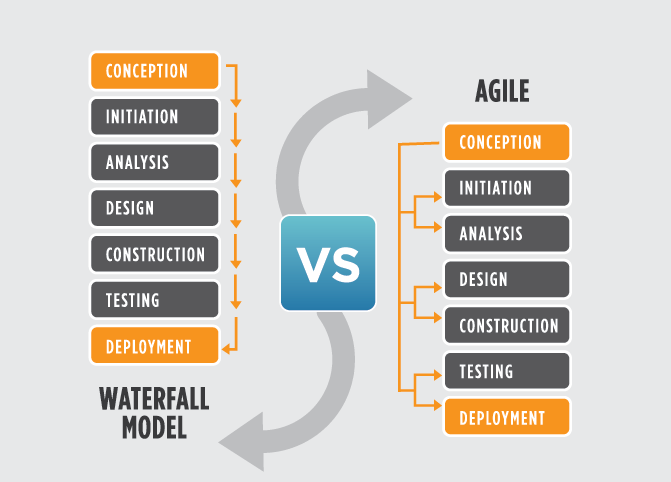
\includegraphics[width=\textwidth, height=150pt]{dissertation/dissertation/img/methodology.png}

\bigskip

In this chapter, the methodologies used to create this project will be discussed. A methodology is a way to plan and control the development process of a software product/project/system \cite{hardgrave2003investigating}. There are a number of methodologies that could have been used, such as Extreme Programming, Rapid Application Development, Lean development or the Waterfall model. For this project, a conclusion was reached that the Agile software development methodology was the most fitting.
\section{Agile Development}
The team members felt that Agile development would be the most effective and efficient way to develop this project. With this approach, requirements and solutions could evolve through collaboration between the two team members.
\bigskip

The first phase in development would be the research phase. Research for this project was an ongoing activity, meaning that as the project was in development, the team was constantly researching how to make it better or how to integrate some new technology. The research for this project is described in much more detail in the \hyperref[sec:MethodologyResearch]{\underline{research}} subsection of this chapter. 

The initial research phase however, involved discussions about what the project would do, what technologies and architecture would be used, and the experiments that would need to be conducted to find this out.
\bigskip

Once the development team had a good idea of what the project would do and how it would be developed, an (initially) vague product backlog was made. This was essentially a to do list of features that the team members wanted the finished product to have.

\bigskip

With a product backlog to reference, the development team began using the Scrum\cite{schwaber1997scrum} model to develop this project in a series of sprints. The individual sprints used in the development of the project are explained in more detail in the \hyperref[sec:MethodologyDevelopmentSprints]{\underline{Development Sprints}} subsection of this paper.
These sprints were time-boxed to three weeks to a month. At the beginning of each sprint, in accordance with the Scrum methodology\cite{schwaber1997scrum}, there was a team meeting. These meetings consisted of both members figuring out how many items of work they can commit to, and to then create a sprint backlog(A list of tasks to perform during the sprint).
\bigskip

During each sprint, team members would aim to to take a small set of features or work items, and bring them to coded and tested functionality. By the end of each sprint, these features would be done, tested and integrated into the evolving project. 
\bigskip

On each day that the team was working on a sprint, both team members would attend a scrum meeting. This meeting usually took about ten to fifteen minutes. This meeting was used for the members to share what they worked on the prior day, what they are currently working on, and to offer advice to each other on what to do moving forward.

These meetings were a very convenient way of synchronizing the work each member was doing during a sprint.

\bigskip
In the middle and at the end of each sprint, the team, along with the project supervisor would meet and conduct a review of the sprint. During this meeting the team would demonstrate to the project supervisor what they are working on, and accept any feedback from the project supervisor that would influence the next sprint.

This feedback loop could sometimes result in changes to the freshly delivered functionality, but it could just as likely result in revising or adding items to the project backlog.

\bigskip
At the end of each sprint, the team would conduct a sprint retrospective\cite{moe2010teamwork}. This would also involve the project supervisor, and is an opportunity to reflect on the sprint that has ended, and identify opportunities to improve.
\section{Version Control}
\label{sec:MethodologyVersionControl}
Throughout the life cycle of this project, the team used GitHub. GitHub is a hosting service for version control. The team initially created a GitHub repository, adding both team members as collaborators to the project. GitHub was found to be an extremely useful tool throughout the project. GitHub was primarily used to manage source code, but other useful GitHub features were used. The 'Wiki' section was used to document a high-level overview about the project, such as how to run/use the project, how it was designed, and it's core principles.

\bigskip
One of these features was GitHub's 'Issues' section. This was used to keep track of known bugs and any issues that was discovered during each sprint. Another feature that was used was the 'Projects' section. This section allowed the team to keep track of what was done and what was yet to be done. This was done in the form of a triage which had four categories (Low priority, High priority, Closed, In Progress).

Once the team had a version of the project running on AWS, any changes that were to be integrated to the current version had to go through a number of steps. Firstly, the new changes would be tested on the developers local machine. If these tests were successful, the changes were pushed to the main branch of the github repository. From here, those changes could be pulled down to a staging area on the AWS remote desktop instance. On this staging area, the project was run on a different port to the current version, to check everything was working. If everything was working, some Angular automated tests were ran against the new version to ensure that no bugs had crept through.

\clearpage

If all of these tests passed, the changes were then migrated to the current version of the working application.

\bigskip

\begin{figure}[H]
    \centering
    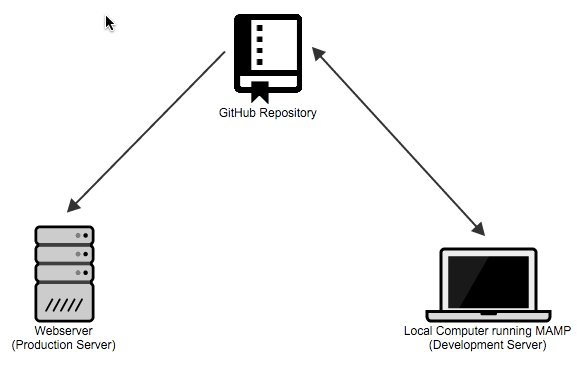
\includegraphics[width=\textwidth, height=200pt]{dissertation/dissertation/img/Control.png}
    \caption{Version Control}
    \label{fig:my_label}
\end{figure}
%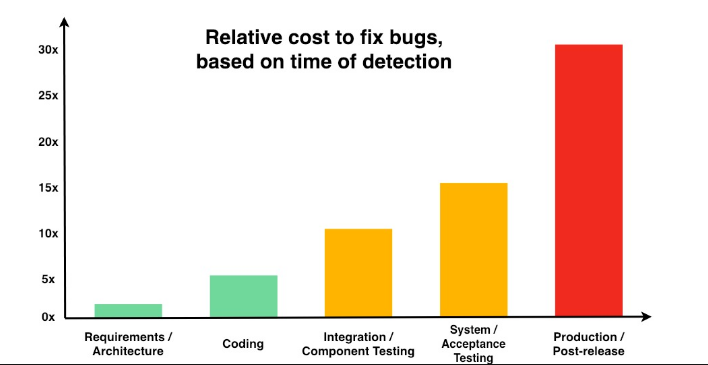
\includegraphics[width=\textwidth, height=180pt]{BugCosts.PNG}


\bigskip
\section{Project Management}
\label{sec:MethodologyProjectManagement}

Project management was a very important aspect of the research and implementation of the project. Project management is important because it ensures there's a proper plan for executing on strategic goals. To keep on track of these goals, the development team created a 'Microsoft Project' schedule. This was used to assign resources to tasks, track progress, and analyse the workload.

\bigskip

This schedule was broken up into phases, with the end of each phase containing a milestone. The team wanted to keep the core credentials of agile development when undergoing the project at hand. It allowed the team to work in sprints for each task, with each task being assigned to either one developer, or both, depending on the scale of the task.

\bigskip

Microsoft Project is quite a unique project management tool in that it offers a number of different views. For instance, you can make use of a Gantt Chart, a resource usage chart, a calendar, and much more. See figures [\ref{fig:my_label1}], [\ref{fig:my_label2}], [\ref{fig:my_label3}], [\ref{fig:my_label4}] below which shows the list of tasks that were undertaken, along with it's corresponding Gantt Chart.

\begin{figure}[H]
    \centering
    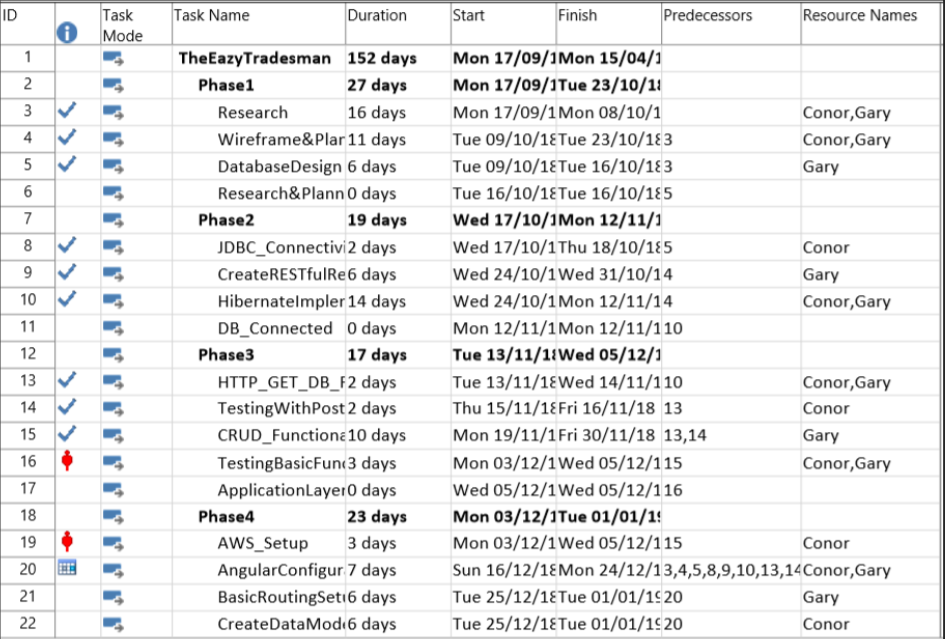
\includegraphics[width=\textwidth, height=180pt]{dissertation/dissertation/img/TaskList1.PNG}
    \caption{Task List: 1}
    \label{fig:my_label1}
\end{figure}
\begin{figure}[H]
    \centering
    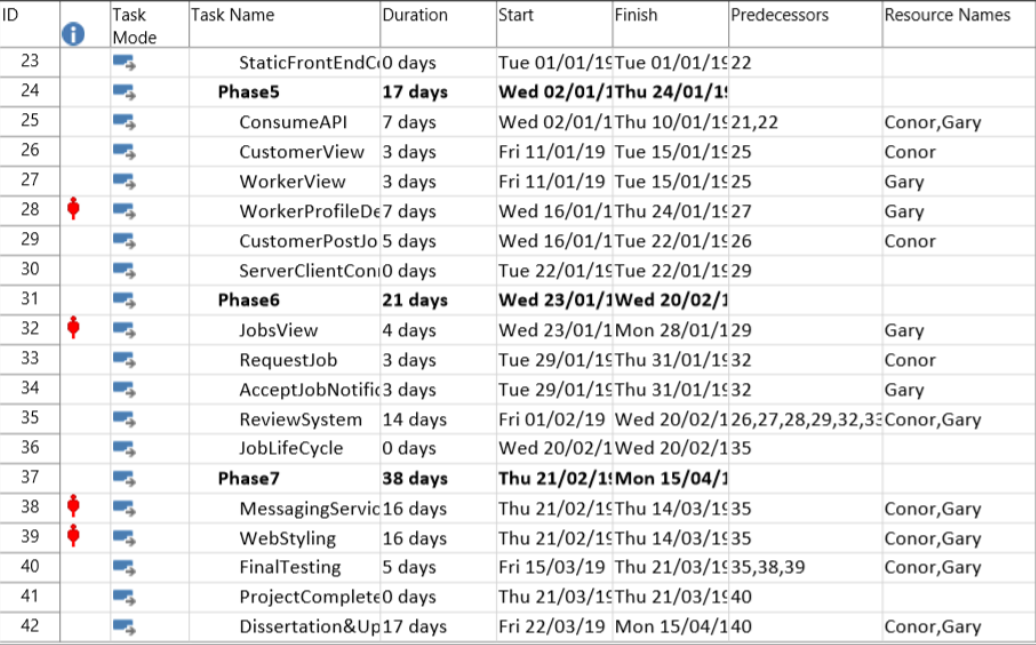
\includegraphics[width=\textwidth, height=180pt]{dissertation/dissertation/img/TaskList2.PNG}
    \caption{Task List: 2}
    \label{fig:my_label2}
\end{figure}
\begin{figure}[H]
    \centering
    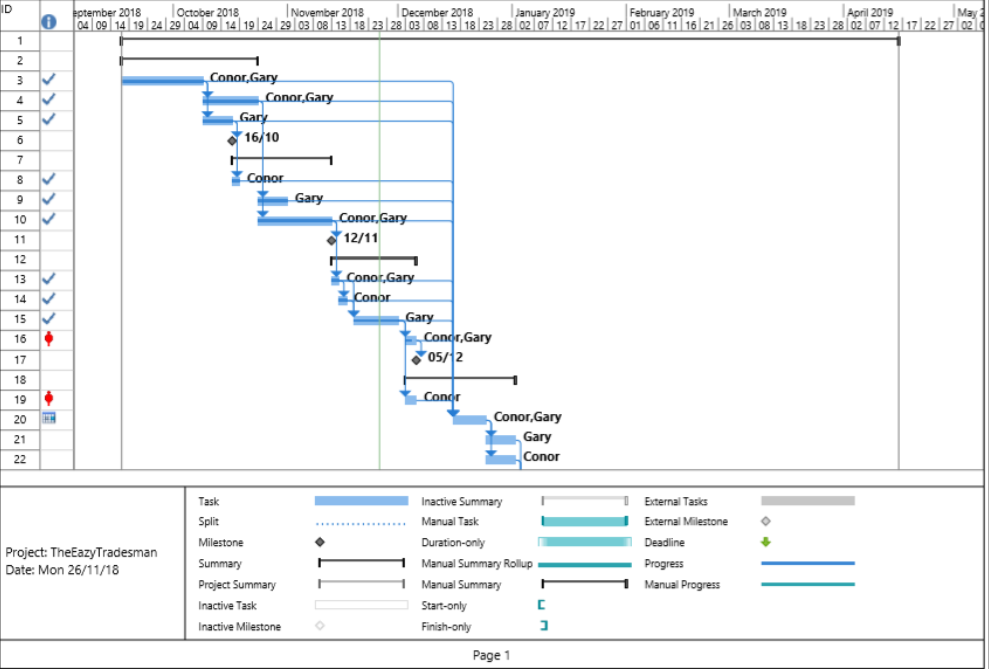
\includegraphics[width=\textwidth, height=180pt]{dissertation/dissertation/img/GanttChart1.PNG}
    \caption{Gantt Chart: 1}
    \label{fig:my_label3}
\end{figure}
\begin{figure}[H]
    \centering
    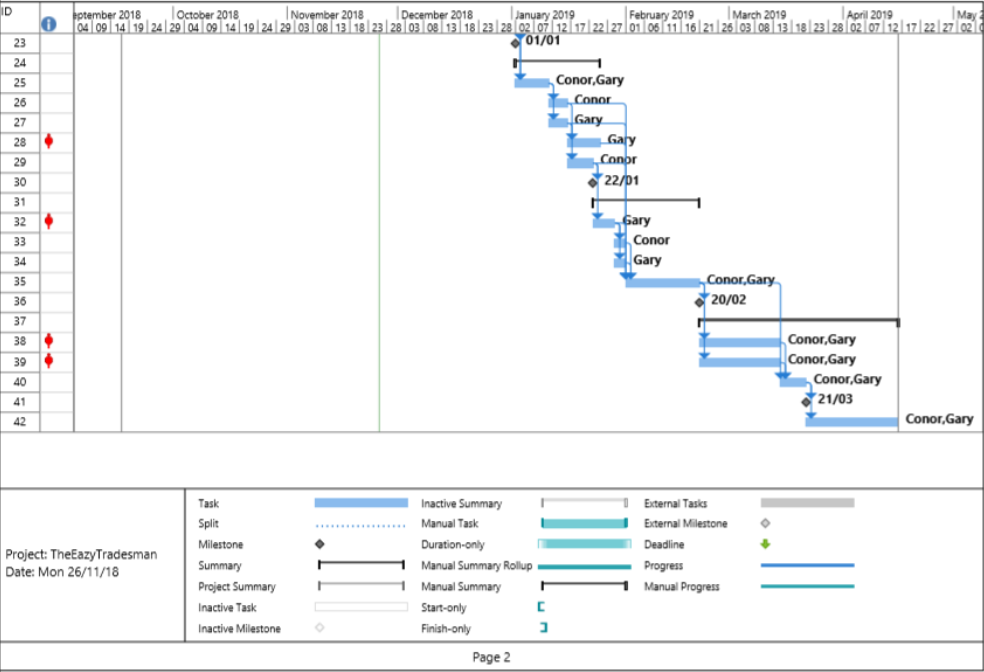
\includegraphics[width=\textwidth, height=180pt]{dissertation/dissertation/img/GanttChart2.PNG}
    \caption{Gantt Chart: 2}
    \label{fig:my_label4}
\end{figure}



\section{Research Phase}
\label{sec:MethodologyResearch}
The research phase incorporated a number of steps and stages. Each stage was critical to achieving an insight into what the project should incorporate and what known issues may arise with the chosen software. Key areas that the team looked at are data and file structure, naming conventions, data integrity, preparing data, variable construction, project documentation and similar products and software.
\subsection{Discussion and Planning}
The first meeting that took place between both members of the team was to decide what technologies should be considered, and what kind of project was going to be developed. 

\bigskip

In order to consider what technologies would be used for this project, there would have to be a general consensus as to what kind of project this was going to be. There were many different avenues to consider. Some of the possibilities included; an AI project with possibly some neural network technology to make classifications or predictions, an advanced game, an application that included Augmented/Virtual/Mixed reality, a web based application focused on using common industry technology with some potentially emerging technology, an application utilising block-chain technology, etc.

\bigskip

In the end, the decision was made to make some sort of web based application that included many common industry technologies, along with trying to integrate a not so common technology that could potentially be used to solve a common industry problem\cite{beeri1979computational}. 

On top of this, discussions took place about what the application would do. After a lot of discussing and debating, it was ultimately decided that an application that gave tradesmen and customers a platform to connect would be a perfect solution. The reason for choosing this, was that it provided an opportunity to incorporate many common industry technologies such as Jax-rs and Angular, along with a not so common technology, Hibernate OGM(Object Grid Mapping). These technologies, and the reasons for using them will be discussed in a lot more detail in the \hyperref[sec:TechnologyReview]{\underline{Technology Review}} chapter of this paper.

This project idea was also interesting to the team because it helps solve the problem of not being able to find a tradesman on time or the problem of a tradesman/woman of not being able to find work in an efficient way. 

Once an idea was in mind for what kind of project was going to be developed and what technologies would be used, experiments needed to be conducted to ensure that this application could in fact be built using the technology the team were considering. These experiments included making a mock-up back end for the project and a mock-up front end to ensure that all of the technologies were indeed compatible. These experiments are outlined in better detail in the next three subsections. 

\subsection{Database Design}
\label{sec:MethodologyDatabaseDesign}
Once the development team had an idea for what the application was going to be able to do, they could now begin designing a database to power this system. From this position, the team members could begin designing the initial draft of the database. 

\bigskip

Customer, Worker, and Job collections were created in a MongoDB database simply called 'todoDB'. At this stage in the experiment, the development team were not concerned with what sort of data these collections were going to hold, only that most application data could be broken into those categories. Each collection only had one field called "name" with a value of the name of the collection eg. "name": "Job".

\bigskip

Once this simple database wire-frame was set up, the team could begin to write queries against the mock data to ensure that the database server was working as expected and that the data could be interacted with. 


\subsection{Wire-frame (Back End)}
\label{sec:MethodologyWireFrame1}
With a simple database in place with some sample data, the development team began creating a mock-up java application to query this data using Hibernate OGM. To achieve this, the team members set up a basic persistence unit to connect with the desired database, and created a java class that could use the hibernate methods to query the sample data on the database. When this data was queried, the results were simply printed to the IDE console. 

\bigskip

When the development team were confident that they could perform CRUD(Create Read Update Delete) operations on the data in the database, they began work creating a simple Jax-rs RESTful service within the same project. This took a bit of more research as it was an area that the development team were previously unfamiliar. A simple REST endpoint was created that could interact with the java controller that could transact with the database. Once a this connection was established, tests could be ran against this endpoint using the REST API testing tool 'Postman'. The \hyperref[sec:TechnologyReviewPostman]{\underline{Postman}} tool will be discussed in much more detail in the \hyperref[sec:TechnologyReview]{\underline{Technology Review}} chapter. 




\subsection{Wire-frame (Front End)}
\label{sec:MethodologyWireFrame2}
With a back-end wire-frame up and running, and that it could perform CRUD operations on very simple data using all of the required technologies, the team got to work making a single page angular web-application that could consume the RESTful service. This involved creating methods that could perform the HTTP GET and HTTP POST transactions with the data in the database. The results of these transactions were simply printed to the browser console. 

\bigskip

Now that the development team had a sample database created with the most necessary data collections, along with a front-to-back end wire-frame in place that could interact with this database, the development team felt they had sufficient research and experimentation completed and could now get started with the development sprints and begin building on this wire-frame.

\section{Development Sprints}
\label{sec:MethodologyDevelopmentSprints}
With the initial experiments conducted, the team now knew what kind of application to make and what technologies to use. From there, the team put together a rough product backlog with features that the project should have. These features were then prioritised and divided up into an initial set of sprints.  These sprints were time-boxed for three weeks to thirty days per sprint. These sprints had the flexibility to change as the project evolved. 

\subsection{Sprint 1: Database Connectivity}
\label{sec:MethodologySprint1}
For the first sprint, after the initial sprint meeting, both members got started on creating a database and connecting it to a java application. During this sprint, the initial database architecture was created. At the same time, a simple java application was created with Maven and then configured with all of the dependencies for Hibernate OGM. Once this was done, the database was connected to the java application. Once the database could be queried from the java application through Hibernate, the data had to be made available to other parts of the application that could handle RESTful requests. 

\bigskip

At the sprint retrospective at the end of the three weeks, the members discussed and investigated how the database architecture might have to change as the project evolves, and whether or not the java application was flexible enough to easily fit an updated database architecture.
\subsection{Sprint 2: Restful Service}
\label{sec:MethodologySprint2}
The next sprint took place after a meeting with the project supervisor to discuss what was achieved in the last sprint. This sprint was concerned with setting up a RESTful service that can access and manipulate the data on the database from an external testing entity. This involved configuring the Java application with Jax-rs, Thorntail(Wildfly-swarm),
and Wildfly(previously known as Jboss). These elements are the dependencies needed to create microservices on a 
"just-enough-appserver". These technologies will be discussed in much more detail in the  \hyperref[sec:TechnologyReviewWildfly]{\underline{Technology Review}}
\bigskip chapter.

With these dependencies in place, a sprint meeting took place to discuss how to create the REST end points and how to connect those end points to the sections of the application that could query the database. 

As these REST endpoints were being set up, they were being tested through the Chrome extension Postman. This tool allowed the team to test GET, PUT, POST and DELETE methods against the database through the RESTful service.
\subsection{Sprint 3: Hosting and Web Navigation}
\label{sec:MethodologySprint3}
To host the website, the team initially used Firebase Hosting service. This brought forward a number of issues. The Bootstrap styling was not being applied when the website was hosted. The website was only being displayed in HTML format. Another issue this created was that the web-page was unable to navigate through each page. This was ultimately down to Firebase Hosting not being able to configure multiple ports. The team needed to use multiple ports for access to the front-end, back-end and the database of the project.

\bigskip

After thorough discussion, the team decided against using Firebase Hosting and decided to use an AWS EC2 Virtual Machine. The reason for this switch was that it allowed for each part of the project to be ran individually. This provided full distribution of the project. AWS also allows for specific port allocation for forwarding and incoming requests. Connection to the front-end application was done using port 4200, with access to the back-end and database done with port 8080.

\bigskip

The web navigation was done 'The angular way', by providing a route to each component in 'app.routes.ts'. This allowed routing to each component/page of the project by including a route in the URL. For example, \begin{verbatim}http://3.16.111.121:4200/login\end{verbatim}.
\subsection{Sprint 4: Initial Front End Configuration}
\label{sec:MethodologySprint4}
To begin front-end development, the team initially configured the login and register web pages. This was done using Firebase Authentication. Firebase Authentication is discussed in detail in the \hyperref[sec:TechnologyReview]{\underline{Technology Review}} Chapter.

\bigskip

When the website is first accessed, the user would be brought to the login page. Here, the user would enter the credentials that they have registered with. These credentials would be checked against the Firebase Authentication users' lists, and if there is a match (and password is correct), the user would be brought to the dummy landing page. If not, the web-page will display an error.

\bigskip

On the login page, there is an option to create an account if the user does not already have an account. When the user clicked on this link, the website would route the user to the register page. On this page, the user would create an account (email address and password). These details would be sent to the Firebase Authentication and stored. The team later added an option to register the user as a customer or worker, but not both.

\subsection{Sprint 5: Front-End and Back-End Connectivity}
\label{sec:MethodologySprint5}
With the initial skeleton of the web application in place and tested, it was time to get started connecting the web app, to the RESTful service back-end. At the sprint meeting at the start of this sprint, members of the team discussed how this might work. This process got the team thinking about the behind the scenes architecture of the web application. It was decided that some sort of MVC(Model View Controller) model would have to be implemented to make this work smoothly. 

\bigskip

Once this architecture was set up, it was time to connect the RESTful service to methods in the controller section of the Angular app. When this was all working, the team could then do a full stack data transfer test by querying some data on the database from the web app and displaying it in the browser console.

\bigskip

At the sprint retrospective, the team members, along with the project supervisor, had a lengthy meeting about the overall trajectory of the project, where the team wanted to take the project, and how the team was going to get there. At this point, the team also started to look at some other functionality that could be added to the application, such as an implementation of the Google Maps API. From this discussion, an updated project backlog was created.


\subsection{Sprint 6: Job Life Cycle and User Permissions}
\label{sec:MethodologySprint6}
At the initial sprint meeting there was a discussion surrounding what the user experiences within the different sections of the application, and how the different types of users navigate the app. Once this was formalised, the different tasks needed to complete this sprint were prioritised and put into a sprint backlog. 

This sprint involved processing job requests on both the customers and workers side of the application, what the different users see when they have an update, how the different users can update their data etc. 

\bigskip

After a mid-sprint meeting, it was decided that extra functionality would be added to stop users from certain accounts accessing certain views. An example of this would be where a customer tries to access a view that only workers are authorised to interact with. The tasks that would be needed to complete this functionality were also prioritised and added to the sprint backlog. 

\bigskip

By the end of this sprint, there was a working prototype of the application up and running that users could interact with. A scrum meeting took place at the end of this sprint, along with the project supervisor to discuss more features that could be added to the product backlog, as well as fleshing out some of the kinks in the current prototype. A discussion also took place about the kind of styling and colour themes that would be applied to the application. 


\subsection{Sprint 7: Styling and Extras}
\label{sec:MethodologySprint7}
With a working prototype of the application up and running on AWS, the development team looked into adding some extra features that could add to the user experience. 

\bigskip

The first of these features to be implemented was the Google Maps API. This API was used to allow customers to attach the location of the job they are posting. With this feature integrated, the workers can view the exact location of a job on Google Maps in order to find out exactly where the job is located. This adds a lot of convenience to the tradesman as it allows them to quickly disregard certain job listings based on their location.

\bigskip

The development team had plans to provide functionality that would allow trade workers to shop for tools and equipment within the application. However, due to severe difficulties during the implementation, this feature had to be abandoned.

\bigskip

Towards the end of this sprint, the team also began adding styling to the application. The goal was to create a theme that is both attractive and practical. Bootstrap and CSS were heavily used to achieve this.
\section{Testing}
\label{sec:MethodologyTesting}
Software testing is an imperative part of any software development methodology\cite{ammann2016introduction}. This process is often skipped, resulting in bug ridden software, and systems that become increasingly complicated and costly to maintain and update. If software bugs are caught in the earlier stages of development, they are much less costly to fix. 

\bigskip

\begin{figure}[h]
    \centering
    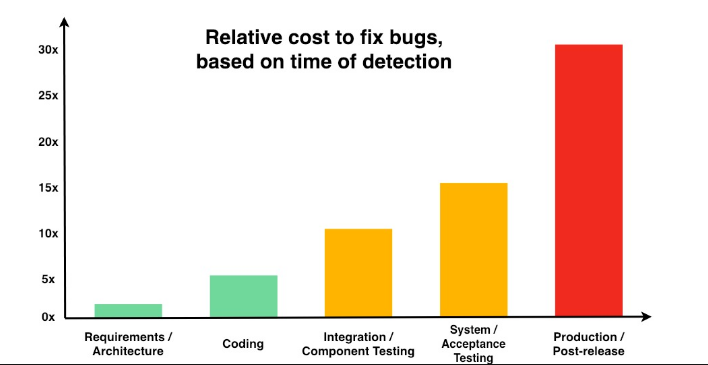
\includegraphics[width=\textwidth, height=180pt]{BugCosts.PNG}
    \caption{Bug Costs}
    \label{fig:bugCosts}
\end{figure}
%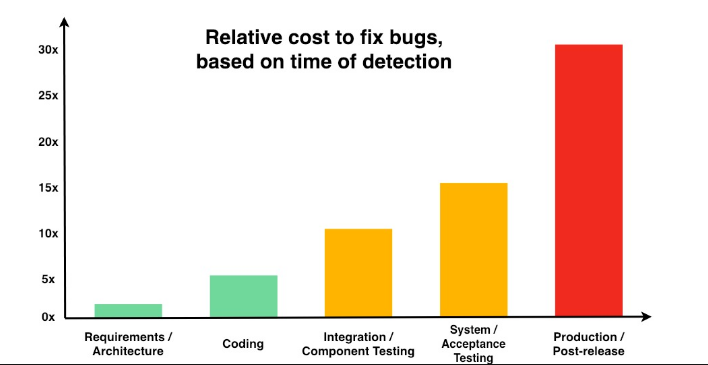
\includegraphics[width=\textwidth, height=180pt]{BugCosts.PNG}


\bigskip

The above graph(fig[\ref{fig:bugCosts}]), is from \href{https://deepsource.io/blog/exponential-cost-of-fixing-bugs/}{\underline{deepsource.io}}.

Testing was a major component in the development of this project. There were both black-box and white-box testing techniques used to ensure the limitation and prevention of bugs in the software. 

\bigskip

\begin{figure}[H]
    \centering
    \includegraphics[width=\textwidth, height=300pt]{dissertation/dissertation/img/BlackWhiteBox.PNG}
    \caption{Black-Box v White-Box Testing}
    \label{fig:whiteBox}
\end{figure}
%\includegraphics[width=\textwidth, height=300pt]{BlackWhiteBox.PNG}

\bigskip

\subsection{Automated Testing (White Box Testing)}
\label{sec:MethodologyWhiteBox}
White-box testing is a testing method in which the tester knows the internal structure and implementation of the software being tested(fig[\ref{fig:whiteBox}]). Examples of white-box testing could be unit tests, integration tests, system tests, or acceptance tests. 

\bigskip

The white-box testing process of testing this project was as follows; Whenever a new feature was added, completed or integrated to the over-all project locally(on the developers device), unit tests were ran against it to ensure it was working as expected. If these tests passed, the new feature would be pushed to the AWS server, and into a staging area.

This staging area can simply be described as running the application on a different port on the server, a port that the users do not have access to. When in this staging area, the same unit tests are ran against the new features. If these tests also pass, it is then pushed to the project running on the public port.

The unit testing tools selected to test this application, were Karma and Jasmine. Karma is a JavaScript test runner created by the AngularJS team. The tests were constructed using the Jasmine framework. Karma provides helpful tools that make it easier to call Jasmine tests while developing the code.

The test specs were designed to thoroughly test the different features in the application, with the knowledge of how these features worked. See fig[\ref{fig:karma}] below for a better idea of what running tests with Karma looks like.

\bigskip

\begin{figure}[H]
    \centering
    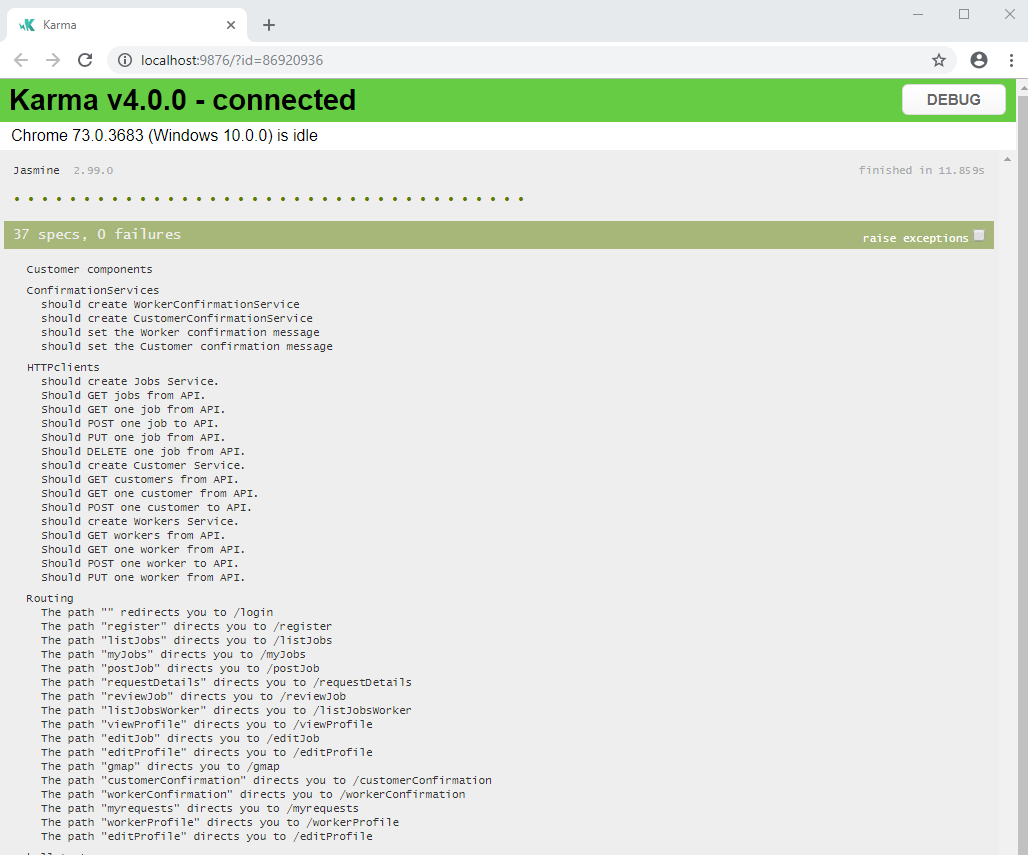
\includegraphics[width=\textwidth, height=300pt]{KarmaTests.PNG}
    \caption{Karma Tests}
    \label{fig:karma}
\end{figure}
%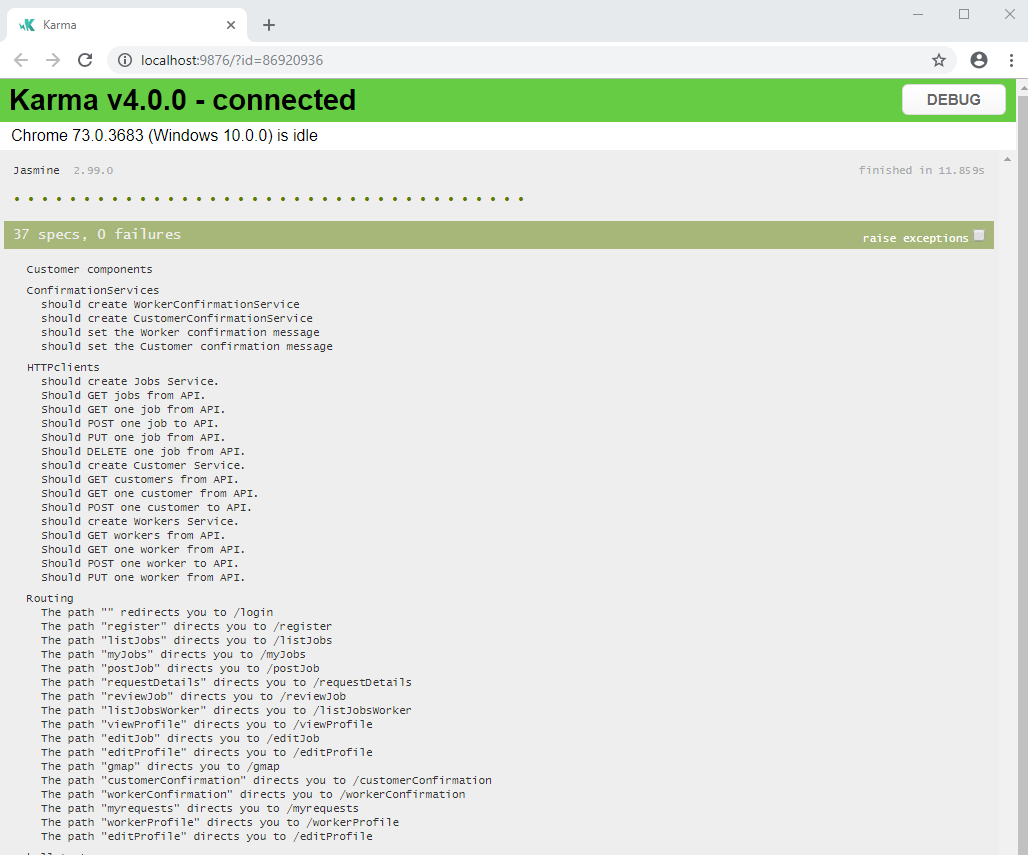
\includegraphics[width=\textwidth, height=300pt]{KarmaTests.PNG}

\bigskip
The tests themselves consist of a set of specifications, these specifications are then checked and if the result is true then the test passes.

\bigskip

Take for example, the third specification under the "ConfirmationServices" test suite. The specification states that
it "should set the Worker confirmation message." The corresponding test that checks whether this specification is true or not looks like fig [\ref{fig:spec}]. 

\bigskip

\begin{figure}[H]
    \centering
    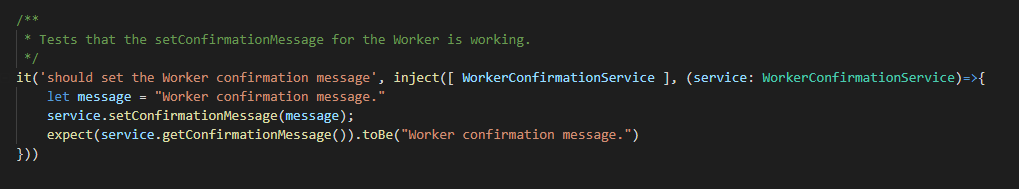
\includegraphics[width=\textwidth, height=80pt]{TestCase.PNG}
    \caption{Karma Specification}
    \label{fig:spec}
\end{figure}
%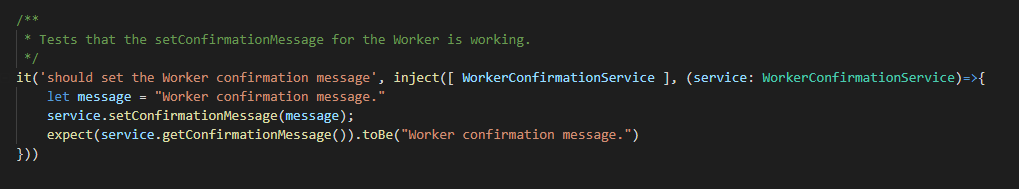
\includegraphics[width=\textwidth, height=100pt]{TestCase.PNG}


\subsection{Black Box Testing}
\label{sec:MethodologyBlackBox}
Black Box Testing, also known as Behavioural Testing, is a software testing method in which the internal structure/design/implementation of the item being tested is not known to the tester. These tests can be functional or non-functional, though usually functional. The development team used Peer testing to test the project.

Peer testing\cite{clark2004peer} is a form of Black Box Testing. In software development, peer review is a type of software review in which a work product (document, code, or other) is examined by its author and one or more colleagues, in order to evaluate its technical content and quality. To perform this, the team allowed peers from the course to test and run the application.

The results of these tests proved invaluable. From these results, the development team found that the application itself was not easy to use. The user found it quite hard to use the functionality of the application without instruction and guidance. For this reason, the development team reviewed the ease of access of the application and adjusted it to suit the needs of the user in terms of website navigation.


\chapter{Technology Review}
\label{sec:TechnologyReview}

\bigskip
\begin{figure}[H]
    \centering
    
\includegraphics[width=\textwidth, height=150pt]{dissertation/dissertation/img/technology.jpg}
    \caption{Technology Review}
    \label{fig:my_label}
\end{figure}
%
\includegraphics[width=\textwidth, height=150pt]{dissertation/dissertation/img/technology.jpg}

\bigskip


\section{Data Tier:}
\label{sec:TechnologyReviewDataTier}

In this section, the technologies that were used in the data layer of the application will be discussed and reviewed in detail. 


\subsection{MongoDB:}
\label{sec:TechnologyReviewMongoDB}

\begin{figure}[H]
    \centering
    
\includegraphics[width=\textwidth, height=150pt]{img/MongoDBLogo.PNG}
    \caption{MongoDB Logo}
    \label{fig:my_label}
\end{figure}
%
\includegraphics[width=\textwidth, height=150pt]{img/MongoDBLogo.PNG}

\bigskip


MongoDB is a cross-platform document oriented database that provides high performance and is easily scalable. 

MongoDB is perfect for applications that involve working with very large amounts of data\cite{moniruzzaman2013nosql}, or where the database needs to be easily scalable. One of the main issues with relational databases (such as MySQL), is that it becomes complicated beyond practicality when the database needs to be scaled. This is because many relational databases were designed to run on a single server. This is a major bottle-neck in the world of computing in the age of big data. 

\bigskip

Big data projects naturally require the data layer to have the ability to scale up and scale out as per demands. This is why NoSQL solutions really seem to be on the rise. MongoDB is one of the most popular and easy to use NoSQL databases.

\bigskip

The main reason that MongoDB was chosen as the database technology for this project, is because the project team believe MongoDB to become increasingly popular and influential in the coming years.

\bigskip
Another reason MongoDB was chosen, is because of the fact that prior to the development of this project, the team members had little experience with MongoDB, and thought that it would be crucial for them to be able to use this technology when they begin to work with industry projects.

\subsubsection{Afterthoughts}
MongoDB proved to be very easy to get set up with and use. The syntax used to read and write MongoDB is called BSON. BSON is also known as "binary JSON" and is very human readable(Looks very similar to JSON syntax).

\bigskip
MongoDB worked well with this project, as all it involved was having a different collection for each of the different categories of data in the application. 

Another reason it fit really well with this project, is because of the fact that this project utilised JSON syntax for transferring the data over HTTP. This meant that the data looked almost the same in transition as it did in the database, making manual testing of the web service much easier.

\bigskip

One pitfall that was experienced with MongoDB is that, because of the document-store nature of the database, there could not be any relationships between the different collections in the database. This made life slightly more complicated because some of the application data was related to multiple collections. For example, each job object had a number of worker objects who requested it. Instead of joining those collections, like one would when using a relational table database, the worker object id's had to be stored as a field in the job object so that the worker collection could then be searched to find the corresponding workers. 

While the work-around was easy, it still made life a bit more complicated during development.

\clearpage

\subsection{Firebase Authentication:}
\label{sec:TechnologyReviewFirebase}
\begin{figure}[H]
    \centering
    
\includegraphics[width=\textwidth, height=150pt]{img/FireBaseLogo.PNG}
    \caption{Firebase Logo}
    \label{fig:my_label}
\end{figure}
Firebase Authentication is a service that can authenticate users using only client-side code. It supports social login providers such as Facebook, GitHub, Twitter and Google. Additionally, it includes a user management system whereby developers can enable user authentication with email and password login stored with Firebase.

\bigskip
Firebase is ideal for web or mobile applications developed with Angular, because it provides highly useful back-end services such as storage, real-time database, authentication, etc. In addition, it is backed by Google and offers a free multi-platform authentication feature.

The Firebase Database is a non-SQL database which works with JSON objects (without tables or records), where it can store and synchronise the data among its users in real-time.

\subsubsection{Afterthoughts}
There are definitely great advantages to using Firebase Authentication.


\begin{itemize}
    \item \textbf{Save time on developing web-service methods for authentication:} Instead, you can just have a method to store user information after user authenticates with Firebase. There is also considerable time saved since you can avoid developing server side methods for different kinds of token verification in case you want to add social logins like Facebook and Google. All of this is handled efficiently with Firebase.
    \item \textbf{Detailed Analytics:} With Firebase authentication, you also get good analytics and demographic information of users.
\end{itemize}


\section{Logic Tier:}
\label{sec:TechnologyReviewLogicTier}
\subsection{Jax-rs:}
\label{sec:TechnologyReviewJax}

\begin{figure}[H]
    \centering
    
\includegraphics[width=\textwidth, height=150pt]{img/Jax-rsLogo.PNG}
    \caption{Jax-rs Logo}
    \label{fig:my_label}
\end{figure}
%
\includegraphics[width=\textwidth, height=150pt]{img/Jax-rsLogo.PNG}

\bigskip

Jax-rs (Java API for RESTful Web Services) is a java programming language API specification that provides support in creating web services in accordance with the REST(Representational State Transfer) architectural pattern. Jax-rs utilises annotations to simplify the creation of RESTful endpoints, making the entire process much more intuitive\cite{burke2009restful}. 

\bigskip

A simplified summary of the specifications are as follows:(The process of creating a REST endpoint will be described in more detail in the \hyperref[sec:SystemDesignLogic]{\underline{Section 4.2 System Design}} chapter of this paper.)


\bigskip
\begin{itemize}
\item @Path specifies the relative path for a resource class or method. 


\item @GET, @PUT, @POST, and @DELETE specify the HTTP request type of a resource.


\item @Produces specifies the response Internet media types.


\item @Consumes specifies the accepted request Internet media types.
\end{itemize}
\bigskip


The reason this specific API was chosen to create the RESTful service part of the project, was the fact that it is the standard API for creating REST endpoints in the Java programming language. This was an important factor because of the fact that creating RESTful services was new to the team. It was considered a wise move to learn how to create RESTful services on a technology the team was already familiar with. 
This is because the Java programming language was the first language that both team members learned, and therefore were more comfortable using it. 

\subsubsection{Afterthoughts}
Jax-rs was the ideal technology to use for the RESTful service segment of the project, because of the fact that the team were already so comfortable with using Java, the learning curve was dramatically cut when learning how to create the RESTful service needed. 

It is also very well documented; any problems that were encountered during the development of the RESTful service were solved remarkably quickly because of the easy to use documentation.

\bigskip

After this project, Jax-rs would be the go-to technology for both team members whenever they need to work with RESTful services in the future.

\subsection{JBoss(Wildfly):}
\label{sec:TechnologyReviewWildfly}

\begin{figure}[H]
    \centering
    
\includegraphics[width=\textwidth, height=150pt]{img/WildFlyLogo.PNG}
    \caption{WildFly Logo}
    \label{fig:my_label}
\end{figure}
%
\includegraphics[width=\textwidth, height=150pt]{img/WildFlyLogo.PNG}
WildFly  is a light weight, flexible Java application server. WildFly is free and open-source.

Previously known as JBoss Application server, it was renamed to WildFly in November 2014. 

\bigskip

The main reason WildFly was chosen as the application server, was simply the fact that the development team had never used it before. The team members had experience using the Apache Tomcat application server, and wanted to have the experience of using something different.

\subsubsection{Afterthoughts}
The application server proved to be very easy to use, with just one command ("java -jar nameOfJar.jar") to start the server running once the Java has been compiled. Both team members would recommend WildFly to anyone, beginner/intermediate/advanced developers, who needed a quick and easy to use application server.



\subsection{Hibernate OGM:}
\label{sec:TechnologyReviewHibernate}
\begin{figure}[H]
    \centering
    
\includegraphics[width=\textwidth, height=150pt]{img/HibernateOGMLogo.png}
    \caption{Hibernate OGM Logo}
    \label{fig:my_label}
\end{figure}
%
\includegraphics[width=\textwidth, height=150pt]{img/HibernateOGMLogo.png}
To understand Hibernate OGM, it is easier to first describe Hibernate ORM. Hibernate ORM(Object Relational Mapping) is a tool for mapping data objects in the Java programming language to a relational database. Hibernate ORM is very commonly used in conjunction with MySQL databases because it offers much more convenient methods of interacting between a database and an application. 

It is this convenience that has caused Hibernate to be heavily adopted into industry operations and software development projects that involve communicating with a relational database. 

\bigskip

In recent years, there has been a big push towards the use of NoSQL databases. This is because of an increasing demand for databases to be scalable, which is a major issue for relational databases. This poses a problem however. The majority of Java EE developers in the world would be used to using SQL databases and now face the task of learning an entirely new skillset of database interactivity with Java. 

\bigskip

Hibernate OGM(Object Grid Mapping) might just solve that problem\cite{storl2015schemaless}. Hibernate OGM reuses Hibernate ORM’s object life cycle management but persists entities into a NoSQL store (key/value, document, column-oriented, etc) instead of a relational database. This means that developers need only be able to use Hibernate/JPA(Java Persistence API) standard, in order to be able to use a whole host of other NoSQL database technologies. 

\bigskip

Hibernate OGM is still a relatively young project, but a very attractive one in today's technological climate.

The main reason Hibernate OGM was used as the persistence engine for this project, was the fact that it offers an easy to use interface between a Java application and a NoSQL database. The development team firmly believe that this is crucial because it allows current developers to adapt to the new database requirements without having to ascend a steep learning curve to learn a new way of interacting with a database from Java.

\subsubsection{Afterthoughts}

Hibernate OGM proved to be extremely intuitive to use, once the developer already has experience working with Hibernate ORM. The basic techniques for persisting and querying data are the same, regardless of whether the database is a SQL or a NoSQL.

\bigskip

The development team, however, did run into issues when trying to map objects that contained arrays. MongoDB does support arrays of objects in collections. When it came time to map these collections to Java objects, errors followed. Because of the fact that OGM is a new concept in relation to ORM, it proved difficult to find solutions to this problem online or in the documentation. This would be one of the drawbacks of using newer technologies. In the end, the team just came up with a work-around(which will be discussed in \hyperref[sec:SystemEvaluationObjectMapping]{\underline{Section 5.6 System Evaulation chapter}} chapter) for the issue as they had to move onto developing other features in the project. 

\bigskip

Overall, Hibernate OGM made life much easier to work with a NoSQL database in conjunction with a Java application and both team members would recommend it to any developers looking to expand on their database skills.


\section{Presentation Tier:}
\label{sec:TechnologyReviewPresentationTier}
\subsection{Angular:}
\label{sec:TechnologyReviewAngular}

\begin{figure}[H]
    \centering
    
\includegraphics[width=\textwidth, height=150pt]{img/Angular6Logo.PNG}
    \caption{Angular 6 Logo}
    \label{fig:my_label}
\end{figure}
%
\includegraphics[width=\textwidth, height=150pt]{img/Angular6Logo.PNG}

\bigskip

Angular is one of the most commonly used platforms for building web applications. Introduced by Google in 2012, Angular is known as the "golden child" among JavaScript frameworks. The angular framework consists of individual components. An example of a component might be a Login page. The component would have a TypeScript file, a HTML file, and a CSS/SCSS file. This completely decouples an application's logic from DOM manipulation.

\bigskip

\begin{figure}[H]
    \centering
    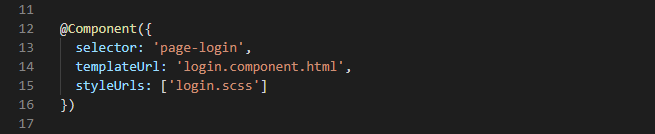
\includegraphics[width=\textwidth, height=100pt]{img/LoginComponent.PNG}
    \caption{Component Example}
    \label{fig:my_label}
\end{figure}
%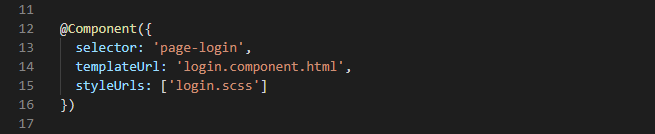
\includegraphics[width=\textwidth, height=100pt]{img/LoginComponent.PNG}

\bigskip

Angular2 was released in 2016, followed by Angular4 by the end of 2016. Angular5 followed in 2017 with Angular6 and Angular7 coming along in 2018. 

\bigskip

The reasoning behind choosing Angular for the development of this project was simple; It was possibly the most popular technology in industry that the team did not previously have any experience with. Angular also uses tools that both team members were already comfortable with, for example HTML and TypeScript. The development team previously had a good wealth of experience using JavaScript, which TypeScript is a syntactical super-set of. 

It also became known to the team, prior to development, that Angular provides tools to help with testing the application such as Jasmine and Protractor. 

Angular was also considered attractive to the team because of the fact that it is "mobile and desktop-ready", meaning that it has one framework for multiple platforms. 

\bigskip

The development team were also aware of the fact that Angular has a large community of active developers. 
This meant that, should any problems arise while using Angular, there would be an abundance of resources to find more information about such problems. 

The simple reason for using Angular version 6 was the fact that at the time of commencing this project, Angular6 was the latest version.

\subsubsection{Afterthoughts}
Angular was an extremely easy piece of technology to get used to. The decoupling of logic and view elements of the application made it really intuitive to create web applications with. 

If a situation arose where a member of the development team was stuck on an issue, or just didn't know how to implement a certain feature in the product backlog, all they had to do was type the specifics of the issue into a browser, and then be greeted with an absolute abundance of possible solutions and answers. 

Both team members would highly recommend learning Angular to any developer at any stage of their career.



\subsection{Bootstrap:}
\label{sec:TechnologyReviewBootstrap}

\begin{figure}[H]
    \centering
    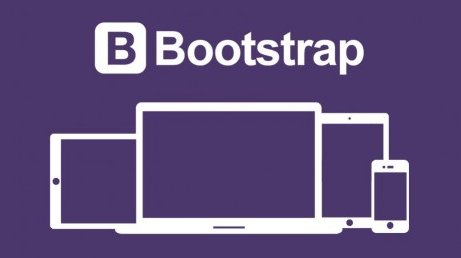
\includegraphics[width=\textwidth, height=150pt]{img/BootStrapLogo.PNG}
    \caption{Bootstrap Logo}
    \label{fig:my_label}
\end{figure}
%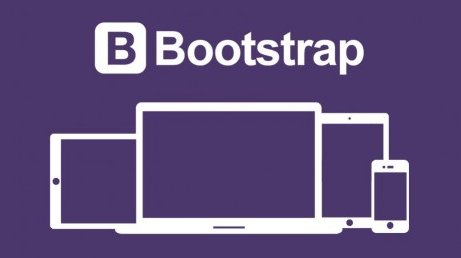
\includegraphics[width=\textwidth, height=150pt]{img/BootStrapLogo.PNG}

\bigskip

Bootstrap is an open-source framework (originally created by Twitter) that one can use as a basis for creating web sites or web applications. Bootstrap contains a combination of JavaScript, HTML, and CSS designed to help build user-interface components for responsive web applications. 

\bigskip

The reasoning behind using Bootsrtap in this project was the fact that it is extremely easy to use and there is an abundance of documentation and resources available for it.

Another reason for choosing Bootstrap as one of the front-end technologies, was the fact that some of the most stylish websites in existence used it. Sites such as Vogue and PopcornTV were built using Bootstrap.  The development team wanted to gain an understanding into how to integrate Bootstrap into potential future projects because of the fact that so many big websites utilise it's features. 

\bigskip

\subsubsection{Afterthoughts}

Bootstrap was a very easy technology to integrate with an Angular front-end application. The documentation was very explanatory and easy for anyone, regardless of whether they would be considered a beginner, intermediate or advanced in software development, to follow. In a very short space of time, anyone could take a very plain front-end application and make it look very professional and slick with the aid of the Bootstrap framework. Both team members would recommend Bootstrap to anyone developing or learning to develop front end web applications. 


 

\section{Languages:}
\label{sec:TechnologyReviewLanguages}
\subsection{Java:}
\label{sec:TechnologyReviewJava}

\begin{figure}[H]
    \centering
    
\includegraphics[width=\textwidth, height=150pt]{img/JavaLogo.PNG}
    \caption{Java Logo}
    \label{fig:my_label}
\end{figure}
%
\includegraphics[width=\textwidth, height=150pt]{img/JavaLogo.PNG}

Java is a very famous and well-rounded multi-purpose programming language and computing platform. It was created by Sun Microsystems in 1995. 

Java is an "object-oriented" programming language, meaning that the language and its' methods are built on the concept of "objects" of data. There are just over nine million Java developers in the world today(2019). 

\bigskip

The Java programming language can be used to create a whole host of applications, mobile apps, desktop apps, web client apps and server side applications. It started with the slogan "Write Once and Run Anywhere" and enables platform independence. Java is present in almost every single area of computer science, from artificial intelligence, to telecommunications, to virtual reality, and shows no signs of slowing down. 

\bigskip

It became clear to both team members at a very early stage of planning and research that Java would be included in this project at some stage. The reason for this, was the fact that both development team members were very experienced in using Java and realised it would be the best option to use for the server-side of the application. 

Java also exposed some nice tools for creating the RESTful service part of the project, Jax-rs, which was covered in an earlier sub-heading. 

\subsubsection{Afterthoughts}
The development team were already very familiar with Java and were very happy with the way it integrated and communicated with the other components in the application. Java is a must-learn for any new developers because the team members feel that, once a new developer learns Java, learning all of the other languages and frameworks becomes much easier as a lot of them are modelled off of the popular programming paradigms present in the Java platform. 



\subsection{Typescript:}
\label{sec:TechnologyReviewTypescript}

\begin{figure}[H]
    \centering
    
\includegraphics[width=\textwidth, height=150pt]{img/TypeScriptLogo.PNG}
    \caption{TypeScript}
    \label{fig:my_label}
\end{figure}
%
\includegraphics[width=\textwidth, height=150pt]{img/TypeScriptLogo.PNG}

\bigskip

TypeScript is an open-source programming language developed and maintained by Microsoft. TypeScript was originally created to bridge the gap between JavaScript and the growing demand for JavaScript to grow into a fully-fledged server-side technology. JavaScript's failure to embrace the features of "Object-Orientation", strong type checking and compile-time error checks prevented JavaScript from succeeding at enterprise level. 

TypeScript is a strongly typed, object-oriented, compiled language. TypeScript is the syntactical super-set of JavaScript, meaning all JavaScript syntax can also be considered TypeScript. TypeScript gets compiled to JavaScript. 

\bigskip

The main reason TypeScript was used for this project is because it works very nicely with Angular. Typescript has also been growing rapidly in popularity over the past number of years. Prior to the development of this application, none of the team members had much experience with TypeScript, but both had quite a bit of exposure to JavaScript. 

\subsubsection{Afterthoughts}

The development team were extremely pleased with how well documented and intuitive writing programs in TypeScript is.  The fact that it is so similar to JavaScript means that any developer who is familiar with writing JavaScript programs can easily make the transition to writing programs in TypeScript. The rise of the Angular framework means that there are more and more developers using TypeScript every day, meaning that anytime the development team ran into problems using TypeScript, there was a lot of resources online to help solve the problems. TypeScript and Angular also make it very easy for developers to integrate third party APIs into the application eg. Firebase, Google-Maps etc.


\subsection{LaTex:}
\label{sec:TechnologyReviewLatex}

\begin{figure}[H]
    \centering
    
\includegraphics[width=\textwidth, height=150pt]{img/LaTexLogo.PNG}
    \caption{Latex Logo}
    \label{fig:my_label}
\end{figure}
%
\includegraphics[width=\textwidth, height=150pt]{img/LaTexLogo.PNG}


Latex is a markup syntax that describes a document's structure and presentation. Latex is typically used in the scientific world to make professional documentation. Technically, LaTex can be considered a programming language because of the fact that it is "Turing Complete"\cite{teller1994turing}, however, it's main job is that of a mark-up language.   

\bigskip

LaTex was used to create the dissertation for this project. The reason the development team decided to use LaTex was the fact that LaTex offers very strong control over the format and structure of a document. 

\section{Development Tools:}
\label{sec:TechnologyReviewDevTools}
\subsection{Git/Github:}
\label{sec:TechnologyReviewGithub}

\begin{figure}[H]
    \centering
    
\includegraphics[width=\textwidth, height=150pt]{img/GitHubLogo.PNG}
    \caption{Github Logo}
    \label{fig:my_label}
\end{figure}
%
\includegraphics[width=\textwidth, height=150pt]{img/GitHubLogo.PNG}

\bigskip

Git is an open-source version control system that was started by the same man who created Linux; Linus Trovalds.

Git is considered, by many, to be the most preferred version control system on the market. A Git "Repository" is simply a directory on a machine that is being tracked by Git. Any changes made to any of the files in this directory can be "added" and then "committed" to the repository. The users have control over what files get added, committed or even tracked by Git within that repository. 

\bigskip

GitHub is a web-based hosting service for version control using Git. Users of Git can create remote versions of their Git repository and "push" changes made in their local repository to the remote repository on the Github servers.  Github has some really nice features including a nice graphical user interface, in contrast to the Git command-line tool. 

Github also makes project collaboration very easy and informed. Github provides the owners of a Github repository with analytics about that repository, such as contributors, clones, traffic etc. 

\bigskip

Git and Github were the obvious version control solutions for this project because of the fact that both team members had previous experience working with the technologies. Git is also one of the most popular version control systems in industry. 

\subsubsection{Afterthoughts}

The development team learned a lot more about how Git and Github works during the course of the development of this application, because of the fact that this was one of the first times they had to collaborate on a Github repository. The team made extensive use of branches to ensure that the development of one feature doesn't affect the development of another. Branches were also used when experimenting with other features without worrying about damaging the master branch. 

The development team, however, did at times find it difficult to resolve merge conflicts and needed the help of Visual Studio Code plugins to solve these difficulties.

\bigskip
Overall, both team members were extremely happy with their use of Git and Github as a well-rounded, well-informed versioning control systems. 



\subsection{Postman:}
\label{sec:TechnologyReviewPostman}

\begin{figure}[H]
    \centering
    
\includegraphics[width=\textwidth, height=150pt]{img/PostManLogo.PNG}
    \caption{Postman Logo}
    \label{fig:my_label}
\end{figure}
%
\includegraphics[width=\textwidth, height=150pt]{img/PostManLogo.PNG}

Postman is a RESTful API testing tool that can be used to inspect API's made by other people, or to test API's developed by oneself. Postman offers a nice user interface that users can utilise to make API requests without needing to write the code to test the API's functionality. 

Users can test GET, PUT, POST, DELETE, and other HTTP requests against an API and view the response in their preferred format. Users can also specify headers on HTTP requests and inspect the intricate details of the returned Response object and payload.

\bigskip

Postman was chosen to test the RESTful service part of this project, because, while the team members had not used it prior to development, they had seen it being used by others and liked how it looked.

\subsubsection{Afterthoughts}
Postman was the perfect tool for testing the RESTful service segment of this project. As the development team was constructing the service, they could test each and every REST endpoint using this tool, and inspect the HTTP Response objects. It also allowed for experimentation to investigate how the client-side application might use headers to heighten security or other features. 

Both team members would, absolutely, use Postman again whenever they are working with RESTful services in the future.


\subsection{Maven:}
\label{sec:TechnologyReviewMaven}

\begin{figure}[H]
    \centering
    
\includegraphics[width=\textwidth, height=150pt]{img/MavenLogo.PNG}
    \caption{Maven Logo}
    \label{fig:my_label}
\end{figure}
%
\includegraphics[width=\textwidth, height=150pt]{img/MavenLogo.PNG}

Maven is a popular build tool used for building Java projects and handling project dependencies. Unlike other tools like Apache Ant, Maven uses conventions and standards for the build procedure, and only requires exceptions to these conventions to be documented in XML files. 

The Maven tool will automatically handle the download of external Java libraries and plug-ins from the Maven repositories, and store them in the local device cache. Maven can also be used to build projects written in C\# or Ruby, but it is primarily used with Java. 

\bigskip

The reason Maven was required in this project development, was the fact that Hibernate OGM and Jax-rs require quite a lot of dependencies, and because of the fact that the team members did not have much prior experience with these technologies. Because of this, they felt it would be wise to allow the Maven tool to handle these dependencies during the build process.

\subsubsection{Afterthoughts}
The development team were very satisfied with how Maven fit into this project. In this instance, Maven was used to build and handle the dependencies for the Java RESTful service. This was the first time the team members have used Maven. They were very pleased to see that one only needed to know a couple of commands in order to integrate Maven into this project, and allow it to mask the complexities of dependency management.

\subsection{Angular CLI:}
\label{sec:TechnologyReviewCLI}

\begin{figure}[H]
    \centering
    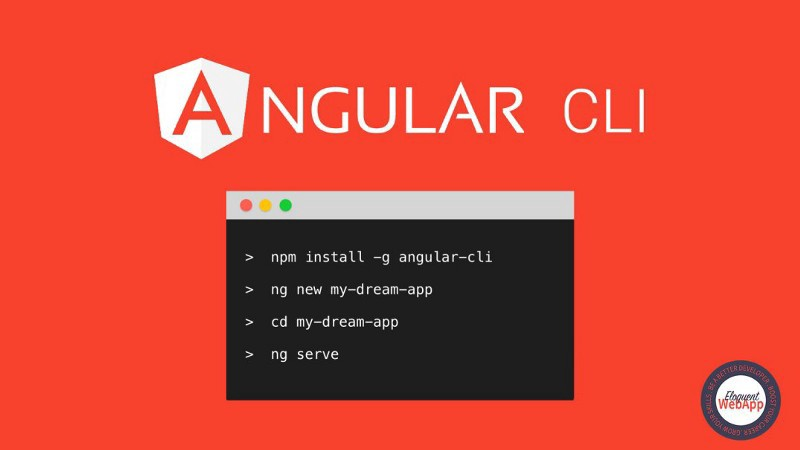
\includegraphics[width=\textwidth, height=150pt]{img/AngularCliLogo.jpeg}
    \caption{Angular CLI Logo}
    \label{fig:my_label}
\end{figure}
%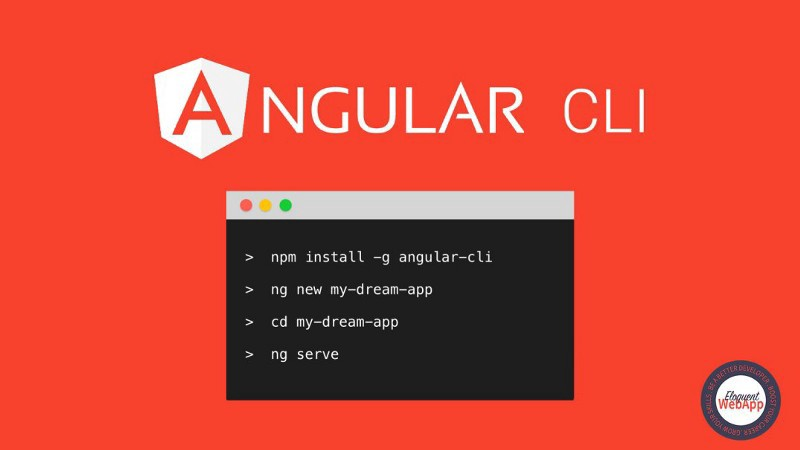
\includegraphics[width=\textwidth, height=150pt]{img/AngularCliLogo.jpeg}

\bigskip

Angular CLI is a command line tool for creating and updating angular apps. CLI stands for command-line-interface. 

When manually creating Angular applications, there is a lot of "boiler plate code" needed to configure the app. Angular CLI solves this problem by creating all of this "boiler plate code" for the developer. For example; if the developer wanted to make an empty component, they would need only type "ng g c myComponent" into the CLI, and the CLI would create a component called myComponent with a ready-to-go HTML file, TypeScript file and CSS/SCSS file. This eliminates the possibility of making silly errors during the creation of component files. CLI also generates the necessary testing files using Jasmine, Karma and Protractor.

\bigskip

The main reason Angular-CLI was chosen as a build tool for this project was the fact that both team members did not have much experience manually creating Angular components from scratch, and didn't want to waste time fixing unforced errors made while configuring the Application. 

\subsubsection{Afterthoughts}
Angular-CLI was an extremely useful tool during the development of this project. The time saved by using CLI to create and modify the Angular application, was put to more productive use in actually developing features in the project, rather than fixing bugs caused by a typo in one of the configuration files. Also, the testing files that CLI automatically brought into the project gave the team a good head-start when the time came to write automated tests for the application. 

\bigskip

Angular CLI is a must-have for developers working with Angular technologies.


\subsection{Karma/Jasmine:}
\label{sec:TechnologyReviewKarma}

\begin{figure}[H]
    \centering
    
\includegraphics[width=\textwidth, height=150pt]{img/JasmineKarmaLogo.PNG}
    \caption{Jasmine and Karma Logos}
    \label{fig:my_label}
\end{figure}
%
\includegraphics[width=\textwidth, height=150pt]{img/JasmineKarmaLogo.PNG}

\bigskip

When creating an Angular application using the Angular-CLI tool, Jasmine and Karma are already resolved and configured for the app.

Jasmine is the framework used to create the tests. It has a lot of functionalities that allow developers to create different kinds of tests.
Karma is a task runner for the Jasmine tests. It uses a configuration file in order to set the startup file, the reporters, the testing framework and the browser among other things.
The default browser used by Karma is Chrome. When the Karma task runner is started, it renders the application tests to the browser as follows:

\begin{figure}[H]
    \centering
    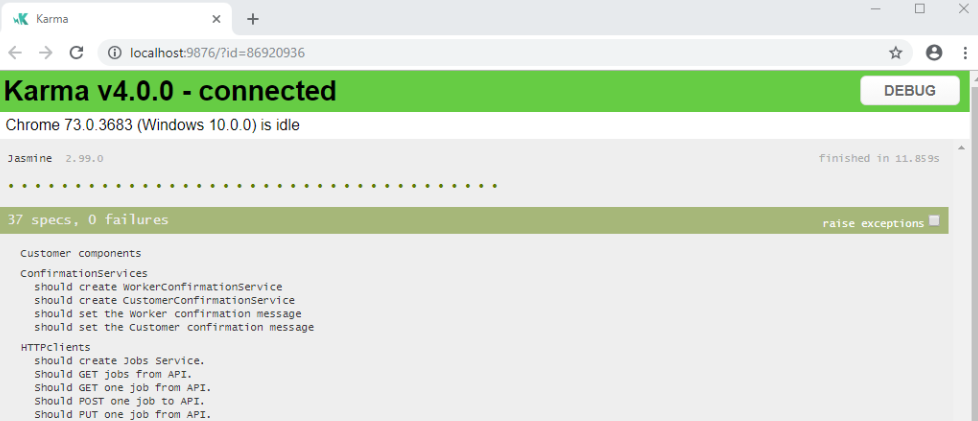
\includegraphics[width=\textwidth, height=150pt]{img/Karma2.PNG}
    \caption{Karma Tests Example}
    \label{fig:my_label}
\end{figure}

%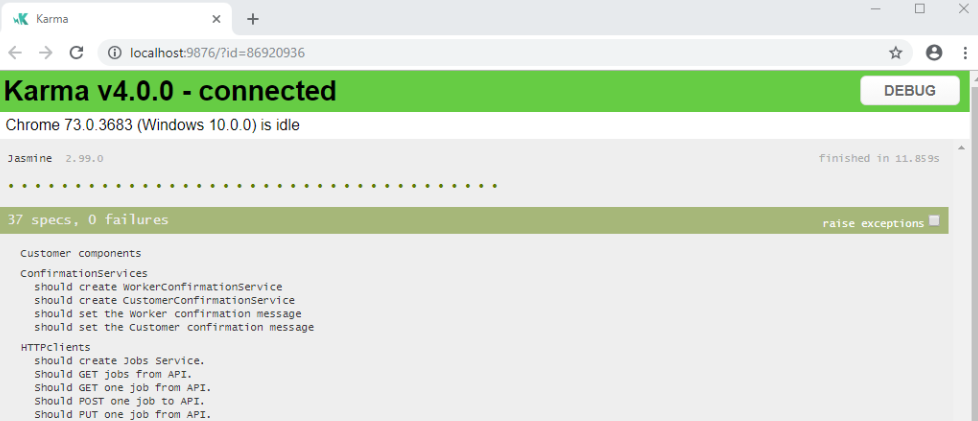
\includegraphics[width=\textwidth, height=150pt]{img/Karma2.PNG}

\bigskip

The main reason for using Jasmine and Karma to do the unit tests on the Angular application, was because of the fact that they were automatically supplied with the app through Angular-CLI. The team investigated online before deciding to use these technologies, to make sure that if any issues were encountered, that there would be enough resources available to resolve those issues. 

\bigskip

\subsubsection{Afterthoughts}

Jasmine and Karma were very well documented and easy to use. Not much automated testing had been done by the development team prior to this project, meaning that Jasmine and Karma would be ideal for developers who do not know a lot about software testing, and wish to learn it.
\subsection{NPM:}
\label{sec:TechnologyReviewNPM}

\begin{figure}[H]
    \centering
    \includegraphics[width=\textwidth, height=150pt]{img/npmLogo.PNG}
    \caption{NPM Logo}
    \label{fig:my_label}
\end{figure}
%\includegraphics[width=\textwidth, height=150pt]{img/npmLogo.PNG}

\bigskip

NPM stands for Node Packet Manager. NPM is a software registry that contains over 800,000 code packages. NPM is open-source and free to use, where developers download all NPM public software packages without any registration or login.

NPM is the default packet manager for the JavaScript run-time environment 'Node.js'. NPM is very commonly used to handle any dependencies involved in creating Angular applications. 

\bigskip

The reason NPM was used as a packet manager in this project, was because NPM works really well in conjunction with Angular applications. Any Angular dependencies that needed to be installed for the application were handled by simply issuing the command - "npm install nameOfPacket". This would automatically handle any background work required for configuring that dependency. 

\subsubsection{Afterthoughts}

NPM was the ideal packet manager for the client-side of the project. Any dependencies that Angular required, regardless of the APIs that were being used, were automatically handled by NPM in the background. If, at any stage, the application was missing dependencies, for example when one team member adds dependencies to their local version of the project and pushes that to Github, could simply be resolved by typing "npm install" into the command line.
\bigskip


\section{Development Environment:}
\bigskip


\subsection{Eclipse:}
\label{sec:TechnologyReviewEclipse}
\begin{figure}[H]
    \centering
    \includegraphics[width=\textwidth, height=150pt]{img/eclipseLogo.png}
    \caption{Eclipse Logo}
    \label{fig:my_label}
\end{figure}
%\includegraphics[width=\textwidth, height=150pt]{img/eclipseLogo.png}

\bigskip

Eclipse IDE is the most widely used IDE for Java. An IDE(Integrated Development Environment) is a piece of software that provides  comprehensive facilities to computer programmers for software development. Eclipse is mainly used to for Java development, but it can also support other programming languages via plug-ins such as C, C\#, C++, Python, Ruby etc. 

\bigskip

Eclipse was used as the IDE for programming the server-side, Java RESTful service part of this project. The reason Eclipse was used, was the fact that both team members had a lot of experience writing Java programs using Eclipse. There really was no reason to use another IDE other than Eclipse to do this job. There was some discussions during the research phase where the team considered using IntelliJ as the IDE for the Java programming. This idea was quickly discontinued because of the fact that the team felt they would be more comfortable using a familiar IDE considering they were going to be using some unfamiliar(to them) technologies.

\subsubsection{Afterthoughts}

The team members were both very content with the Eclipse IDE because it made the newer technologies they were using, such as Jax-rs and Hibernate OGM, feel that little bit more familiar and understandable to them when using these new technologies through a familiar IDE.


\subsection{Visual Studio Code:}
\label{sec:TechnologyReviewVSC}
\begin{figure}[H]
    \centering
    \includegraphics[width=\textwidth, height=150pt]{img/vscLogo.PNG}
    \caption{Visual Studio Code Logo}
    \label{fig:my_label}
\end{figure}
%\includegraphics[width=\textwidth, height=150pt]{img/vscLogo.PNG}

\bigskip

Visual Studio Code(VSC) is a popular IDE developed by Microsoft. Visual Studio Code provides support for debugging, embedded Git control, syntax highlighting, intelligent code completion, and more.

\bigskip

VSC was selected as the source code editor for the Angular front-end faction of the project. The reason for this, was the fact that up to the point of developing this project, the team members didn't have much exposure to VSC and were curious to try it because it seemed to be so popular amongst the software community. 

\subsubsection{Afterthoughts}

Visual Studio Code turned out to be a very useful code editor. The integrated Git control and intelligent code completion made coding with it very efficient. VSC also has a nice feature included that makes refactoring code really simple and quick.

Both team members would highly recommend Visual Studio Code to any developers looking to develop software in Angular, or for that matter, any framework or programming language. 

\subsection{Overleaf:}
\label{sec:TechnologyReviewOverleaf}
\begin{figure}[H]
    \centering
    \includegraphics[width=\textwidth, height=120pt]{img/overleafLogo.png}
    \caption{Overleaf Logo}
    \label{fig:my_label}
\end{figure}
%\includegraphics[width=\textwidth, height=120pt]{img/overleafLogo.png}

Overleaf provides a web-based freemium academic writing environment. Overleaf allows users to create a range of documents such as blog posts, journal articles, etc. Overleaf provides a lot of rich features that make it very convenient to write and create documents in LaTex syntax without much prior knowledge of LaTex.

\bigskip

In this project, Overleaf was used as the online text editor to create and write the entire dissertation. Overleaf also provides collaboration services meaning that both team members could work on the same document concurrently.


\subsection{AWS Cloud Platform:}
\label{sec:TechnologyReviewAWS}

\begin{figure}[H]
    \centering
    \includegraphics[width=\textwidth, height=120pt]{img/awsLogo.PNG}
    \caption{AWS Cloud Logo}
    \label{fig:my_label}
\end{figure}
To host the dynamic website application, the team used an AWS EC2 Virtual Machine. An EC2 instance is a virtual server in Amazon’s Elastic Compute Cloud (EC2) for running applications on the Amazon Web Services (AWS) infrastructure. Amazon provides a variety of types of instances with different configurations of CPU, memory, storage, and networking resources to suit user needs. Each type is also available in two different sizes to address workload requirements.

\bigskip

The AWS Platform was chosen for its scalability, flexibility, and reliability. The team wanted to show that the project can be completely distributed, with the front-end services and back-end services being executed independently of each other. AWS provided the suitable tools to get this done.


\subsubsection{Afterthoughts}
In the beginning, the team ran into issues concerning the port forwarding. There is a substantial amount of configuration required to set up the ports correctly, such as selecting the correct port, and allowing the correct type of traffic through the firewall (HTTP, TCP). AWS itself, is easy to use, has no capacity limits, provides speed and agility, and is secure and reliable. Overall, the team were content with the AWS Cloud Platform.

\chapter{System Design}
\label{sec:SystemDesign}


\begin{figure}[H]
    \centering
    \includegraphics[width=\textwidth, height=170pt]{dissertation/dissertation/img/Architecture.png}
    \caption{System Design}
    \label{fig:my_label}
\end{figure}
%\includegraphics[width=\textwidth, height=150pt]{dissertation/dissertation/img/systemDesign.png}

\bigskip
In this chapter of the document, the overall design and architecture of the project will be discussed.  This will be achieved through code snippets, UML diagrams, abstract architecture diagrams and literal explanations. This chapter will be broken up into four sections; the  \hyperref[sec:SystemDesignDataTier]{\underline{Data Tier}}, \hyperref[sec:SystemDesignLogic]{\underline{Logic Tier}}, \hyperref[sec:SystemDesignPresentationTier]{\underline{Presentation Tier}}, and \hyperref[sec:SystemDesignHosting]{\underline{Hosting}}. The Data Tier section describes the system design behind the factions of the application that store and manage data. The Logic Tier section describes how data flows through the application to get to and from the Data Tier, and to and from the Presentation Tier, as well as how that data is manipulated along the way. The Present Tier section describes what happens to the data once it reaches the client, as well as how the client can interact with the data and application as a whole. The Hosting section describes how the application is hosted, and the changes that needed to be made to the application to make that possible.


\section{Data Tier}
\label{sec:SystemDesignDataTier}

\bigskip

The Data Tier is a catch-all phrase used to describe any mechanism used to allow for the storage and manipulation of data in the application. More often than not, these mechanisms are databases. 

There were two databases used in the design of this application; MongoDB, and Firebase.
The motives for using these databases are described in more detail in the \hyperref[sec:TechnologyReview]{\underline{Technology Review}} chapter of this paper.


\subsection{MongoDB}
\label{sec:SystemDesignMongoDB}

\bigskip

MongoDB was used to store all of the user data that was not related to authentication data. The MongoDB technology was discussed in an earlier chapter, but as a quick summary, MongoDB stores data in groups called collections. Each collection is completely independent (Unlike MySQL where tables can be joined.) 

\bigskip

Three collections were used for the database on this occasion; a Customer collection, a Worker collection, and a Job collection. 

Each object in a collection is stored as BSON(Binary JSON). The schema for each collection looks like fig[\ref{fig:workerSchema}]. 

\subsubsection{Worker Schema}
\label{sec:SystemDesignWorkerSchema}

\begin{figure}[H]
    \centering
    \includegraphics[width=150pt, height=150pt]{DesignImages/WorkerSchema.PNG}
    \caption{Worker Schema}
    \label{fig:workerSchema}
\end{figure}
%\includegraphics[width=150pt, height=150pt]{DesignImages/WorkerSchema.PNG}

\bigskip

An example Worker object might look like fig[\ref{fig:workerExample}].
\begin{figure}[H]
    \centering
    \includegraphics[width=\textwidth, height=150pt]{DesignImages/WorkerObject.PNG}
    \caption{Worker Example}
    \label{fig:workerExample}
\end{figure}
%\includegraphics[width=\textwidth, height=150pt]{DesignImages/WorkerObject.PNG}

\bigskip

\begin{itemize}

\item "id": Refers to the unique Mongo identifier for this object. This ID is automatically generated by the MongoDB engine when the object is created on the database.

\item "firstName": A string data-type that simply refers to the first name of the worker.

\item "secondName": A string data-type that simply refers to the second name of the worker.

\item "address": A string data-type that refers to the address of the workers operation.

\item "age": An integer data-type that refers to the age of the worker.

\item  "trade":  A string data-type that refers to the trade/s of the worker.

\item "rating": A string data-type that refers to the rating of the worker*. 

\item "phoneNumber": A string data-type that refers to the phone number/other contact information for the worker.

\item "email": A string data-type that refers to the email address of the worker object.

\item "website": A string data-type that refers to the website of the worker. 

\item "firebaseUid": A string data-type that refers to the Firebase UID for the worker. This value is used to check if the user exists on the Firebase database when the user is logging in.

\item "jobRequests": A string data-type that refers to a list of blank space separated values, representing the Mongo identifiers for the jobs the worker has requested.

\item "jobAccepted": A string data-type that refers to a list of blank space separated values, representing the Mongo identifiers for the jobs the worker has requested, that have been accepted by the corresponding customer.
\end{itemize}

* The reason that the "rating" field needs to be a string data-type, is the fact that the rating field doesn't store the actual rating for the worker. This field stores a string of two comma separated values. The first value is the amount of ratings this worker has had, and the second value represents the total of all of the ratings for that worker. 

If the worker has been rated three times, and each rating was 50, 75 and 100 respectively, the value of the "rating" field would be "3, 225"(50+75+100). The ratings are handled in this way, so that another field is not needed on the database to store the total amount of ratings, so that an average can be calculated. On the client side, this string is split by the comma, and the second value is simply divided by the first value, then rounded to the nearest integer for the actual rating to be displayed.
\bigskip

\subsubsection{Customer Schema}
\label{sec:SystemDesignCustomerSchema}

\begin{figure}[H]
    \centering
    \includegraphics[width=150pt, height=130pt]{DesignImages/CustomerSchema.PNG}
    \caption{Customer Schema}
    \label{fig:my_label}
\end{figure}
%\includegraphics[width=150pt, height=130pt]{DesignImages/CustomerSchema.PNG}

\bigskip

An example Customer object might look like fig[\ref{fig:customerExample}].

\begin{figure}[H]
    \centering
    \includegraphics[width=220pt, height=130pt]{DesignImages/CustomerObject.PNG}
    \caption{Customer Example}
    \label{fig:customerExample}
\end{figure}
%\includegraphics[width=220pt, height=130pt]{DesignImages/CustomerObject.PNG}

\bigskip

\begin{itemize}

\item "id": Refers to the unique Mongo identifier for this object. This ID is automatically generated by the MongoDB engine when the object is created on the database.

\item "firstName": A string data-type that simply refers to the first name of the customer.

\item "secondName": A string data-type that simply refers to the second name of the customer.

\item "address": A string data-type that refers to the address of the customers residence. 

\item "age": An integer data-type that refers to the age of the customer.

\item "firebaseUid": A string data-type that refers to the Firebase UID for the customer. This value is used to check if the user exists on the Firebase database when the user is logging in.

\end{itemize}
\bigskip

\subsubsection{Job Schema}
\label{sec:SystemDesignJobSchema}

\begin{figure}[H]
    \centering
    \includegraphics[width=150pt, height=150pt]{DesignImages/JobSchema.PNG}
    \caption{Job Schema}
    \label{fig:my_label}
\end{figure}
%\includegraphics[width=150pt, height=150pt]{DesignImages/JobSchema.PNG}

\bigskip

An example Job object might look like fig[\ref{fig:jobExample}].
\begin{figure}[H]
    \centering
    \includegraphics[width=\textwidth, height=150pt]{DesignImages/JobObject.PNG}
    \caption{Job Example}
    \label{fig:jobExample}
\end{figure}
%\includegraphics[width=\textwidth, height=150pt]{DesignImages/JobObject.PNG}

\bigskip

\begin{itemize}

\item "id": Refers to the unique Mongo identifier for this object. This ID is automatically generated by the MongoDB engine when the object is created on the database.

\item "trade": A string data-type that simply refers to the trade/s needed to complete this job. 

\item "description": A string data-type that refers to a description of this job.

\item "customer": A string data-type representing the MongoDB id reference to the customer that posted this job.

\item "requests": A string data-type that contains a list of space separated values, each of which represent the MongoDB id reference to a worker that requested this job.

\item "location": A string data-type that refers to the location of the job.

\item "date": A string data-type that is automatically generated when the job is created, representing the date that the job was posted.

\item "contact": A string data-type referring to any contact information the customer puts on the job post eg. name, phone number, email etc.

\item "complete": A boolean data-type that refers to whether or not the job has been completed.

\item "accepted": A boolean data-type that refers to whether or not any requests on this job have been accepted.

\end{itemize}

\subsection{Firebase}
\label{sec:SystemDesignFirebase}
Using Firebase Authentication is relatively simple. To sign a user into your app, you first get authentication credentials from the user. These credentials can be the user's email address and password, or an OAuth token from a federated identity provider. Then, you pass these credentials to the Firebase Authentication SDK. The backend services will then verify those credentials and return a response to the client. The users details are stored within the Firebase Authentication Database, with the users password being securely hashed, as seen in fig [\ref{fig:listUsers}].

\begin{figure}[H]
    \centering
    \includegraphics[width=\textwidth, height=90pt]{dissertation/dissertation/img/firebaseUsers.PNG}
    \caption{List of Users}
    \label{fig:listUsers}
\end{figure}


After a successful sign in, you can access the user's basic profile information, and you can control the user's access to data stored in other Firebase products. You then use the provided authentication token to verify the identity of users in your own backend services.


\section{Logic Tier}
\label{sec:SystemDesignLogic}

The logic tier of this project consisted of Java, Hibernate OGM, and Jax-rs. These technologies were described in more detail in the last chapter. 

The logic tier deals with getting information to and from the database. It then does some processing on that data, before sending a result/response back to a client via the RESTful endpoints. The different components involved in this transaction of data will be discussed here. 

\subsection{Database Connectivity}
\label{sec:SystemDesignDatabaseConnectivity}

\bigskip

When using Hibernate to handle the object mapping to the database, a configuration file needs to be created in order to tell that Java program what database to connect to. This configuration file is called "persistence.xml".

\bigskip

This "persistence.xml" file is where the persistence units are initialised. The persistence.xml file in this project only has one persistence unit because it only needs to transact with one database.

\begin{figure}[H]
    \centering
    \includegraphics[width=\textwidth, height=150pt]{DesignImages/persistence.PNG}
    \caption{Persistence.xml}
    \label{fig:my_label}
\end{figure}
%\includegraphics[width=\textwidth, height=150pt]{DesignImages/persistence.PNG}

\bigskip

This persistence unit describes everything the Java program needs to know about the database in question. The first thing it does, is it states the Java classes that will be used to map objects from the database onto. These classes are surrounded by the $\langle class \rangle$ $\langle /class \rangle$ tags. 

\bigskip

The next segment of the persistence unit is the segment that describes the actual properties of the database to connect with. The properties of this database are surrounded in the $\langle property/ \rangle$  tags, in this case "todoDB" would be the name of the database to connect with. Other properties such as "host" describe where the database is running, "username", and "password" describe the user name and password to gain access to the database.

\bigskip

Now that a connection to the database has been configured, the Java application can query it using the Hibernate methods.

\subsection{Models}
\label{sec:SystemDesignModels}

There are three models in the Java application, one for each collection in the database. These models should be designed in such a way, that it is easy for the Hibernate engine to map between the Java and BSON(MongoDB representations of an object) objects.

\subsubsection{Job}
\label{sec:SystemDesignJob}

The Job model is designed as seen in fig[\ref{fig:jobModel}]. 

\begin{figure}[H]
    \centering
    \includegraphics[width=\textwidth, height=180pt]{DesignImages/JobModel.PNG}
    \caption{Job Model}
    \label{fig:jobModel}
\end{figure}
%\includegraphics[width=\textwidth, height=160pt]{DesignImages/JobModel.PNG}

\bigskip

The field names and types on this model allow for an easy mapping to and from the BSON representation of the "Job" collection. This model is annotated with @Entity, signifying that this object will be an entity in the database. The @NamedQuery annotation allows one to create their own query and map that query to an actual Hibernate query.

\subsubsection{Worker}
\label{sec:SystemDesignWorker}

The Worker model is designed as seen in fig[\ref{fig:workerModel}].

\begin{figure}[H]
    \centering
    \includegraphics[width=\textwidth, height=200pt]{DesignImages/WorkerModel.PNG}
    \caption{Worker Model}
    \label{fig:workerModel}
\end{figure}
%\includegraphics[width=\textwidth, height=160pt]{DesignImages/WorkerModel.PNG}



\subsubsection{Customer}
\label{sec:SystemDesignCustomer}

The Customer model is designed as seen in fig[\ref{fig:customerModel}].

\begin{figure}[H]
    \centering
    \includegraphics[width=\textwidth, height=160pt]{DesignImages/CustomerModel.PNG}
    \caption{Customer Model}
    \label{fig:customerModel}
\end{figure}
%\includegraphics[width=\textwidth, height=160pt]{DesignImages/CustomerModel.PNG}

\bigskip

All of the models in this project needed to be designed in a way that can be easily mapped back and forth from the database. This caused some issues in this project. These issues will be discussed in detail in a later \hyperref[sec:SystemEvaluationObjectMapping]{\underline{chapter}}.



\subsection{Controllers}
\label{sec:SystemDesignControllers}

In this application, a set of controller classes were used to deal with the data transfer between the REST endpoints and the database.  There are three controller classes used in this project. One controller class to interact between the Worker RESTful endpoints and the worker collection in the database, another controller to interact between the Job RESTful endpoints and the job collection in the database, and another controller to interact with the Customer RESTful endpoints and the customer collection in the database.

\bigskip

To explain how this transaction of data works, code snippets will be provided. There will be an example of how a controller(job controller) gets data from the database, and how the same controller sends data to the database.



\subsubsection{From Database}
\label{sec:SystemDesignDatabase}

Below(fig[\ref{fig:findJob}]) is an example of how a single job object can be retrieved from the database, given the id of the job.

\begin{figure}[H]
    \centering
    \includegraphics[width=\textwidth, height=140pt]{DesignImages/JobGetData.PNG}
    \caption{Find Job}
    \label{fig:findJob}
\end{figure}
%\includegraphics[width=\textwidth, height=140pt]{DesignImages/JobGetData.PNG}

\bigskip

The "em" object that is called in this method is an EntityManager. This EntityManager class handles the connections and mapping to and from the database. In this instance, the Job model class is being passed in, as well as the id. This means that the EntityManager will now find the collection that is mapped to the Job class, find the object in that collection with the given id, map that object to an object of the Job java class and return that object.

This object gets returned to the job REST end point.

\subsubsection{To Database}
\label{sec:SystemDesignToDatabase}
Below(fig[\ref{fig:create}]) is an example of how a single job object can be created on the database, given the job object to be created.

\begin{figure}[H]
    \centering
    \includegraphics[width=\textwidth, height=140pt]{DesignImages/JobPutData.PNG}
    \caption{Persist Job}
    \label{fig:create}
\end{figure}
%\includegraphics[width=\textwidth, height=140pt]{DesignImages/JobPutData.PNG}

\bigskip

Whenever the Java application needs to add something, or update something on the database, it needs to start a transaction. This transaction, in simple words, is to prevent other entities from writing to the same piece of data at the same time as this would result in ambiguity.  

Once the data has been written to the database, the transaction needs to be ended so that other entities can now write to that same piece of data. 

\bigskip

The "em.persist" method is a Hibernate method which is used to create a new object on the database. If this was an update method, this persist would change to "em.merge(job)".
\subsection{REST Endpoints}
\label{sec:SystemDesignEndPoints}

The REST endpoints refer to the methods in the application that allow a third-party client application to interact(Create, Read, Update and Delete) with the data in the database. As mentioned in the \hyperref[sec:TechnologyReviewJax]{\underline{Technology Review}} chapter, Jax-rs was the technology used to allow for this interaction. 

\bigskip

Jax-rs allows for the mapping between HTTP methods, and java methods. The typical HTTP methods are GET, PUT, POST, DELETE. In this project, the HTTP GET method was mapped to a method that allows the reading of data from the database. The HTTP PUT method was mapped to a method to allow for the modification of data in the database. The HTTP POST method was mapped to a method that allows for the creation of new data in the database. The HTTP DELETE method was mapped to a method that allows for the deletion of data from the database. With the mappings done this way, the HTTP client now had full CRUD functionality with the application.

To explain how these mappings work, code snippets will be provided. The code snippets below describe how a HTTP GET and POST method can be mapped to java methods that then call methods in the controller.


\subsubsection{HTTP GET}
\label{sec:SystemDesignGET}

Below(fig[\ref{fig:httpGET}]) is an example of how a HTTP GET method can be mapped to a java method that then fetches a Job object from the controller class.

\begin{figure}[H]
    \centering
    \includegraphics[width=\textwidth, height=150pt]{DesignImages/JobGET.PNG}
    \caption{HTTP GET Job}
    \label{fig:httpGET}
\end{figure}
%\includegraphics[width=\textwidth, height=150pt]{DesignImages/JobGET.PNG}

\bigskip

The @GET annotation is what maps this method to a HTTP GET method for the job resource. The @Path annotation means that the variable inside the curly braces will be passed in to this method as a parameter that came from the path the client is searching for. In this instance, the path is the id. This id refers to the id of the Job object the client is requesting. This id is then taken and passed in as a parameter to the "findById()" fig[\ref{fig:findJob}] method in the job controller class. The Job object that gets returned by the controller then gets converted to JSON and is returned to the client.

The annotation @Produces(Application.JSON) at the top of the resource class specifies that the Response object is in JSON format.



\subsubsection{HTTP POST}
\label{sec:SystemDesignPOST}

Below(fig[\ref{fig:postHTTP}]) is an example of how a HTTP POST method can be mapped to a java method that allows for the creation of a new Job object in the database.

\begin{figure}[H]
    \centering
    \includegraphics[width=350pt, height=170pt]{DesignImages/JobPOST.PNG}
    \caption{HTTP POST Job}
    \label{fig:postHTTP}
\end{figure}
%\includegraphics[width=350pt, height=170pt]{DesignImages/JobPOST.PNG}

\bigskip

The @POST annotation is what maps a HTTP POST method to this method for the job resource. This method takes in a Job object as an input parameter. After performing some basic client authentication(which will be discussed in a later chapter), the "create(job)" fig[\ref{fig:create}] method is called in the job controller class. The is the method that then persists this job object to the database. If this transaction is successful, a HTTP status code "200" is sent back to the client, letting the client know that the transaction was successfully completed.


\section{Presentation Tier}
\label{sec:SystemDesignPresentationTier}

The presentation tier of the application is the tier that the users of the application interact with. The presentation tier deals with processing the users interactions and sending the data for those transactions to and from the RESTful service. As discussed in the Technology Review chapter, the  \hyperref[sec:TechnologyReviewPresentationTier]{\underline{Angular}} framework was used to create the client side application. Typescript was used with Angular, which provides some very intuitive methods for interacting with RESTful services. The presentation tier consists of three segments; The \hyperref[sec:SystemDesignRESTConsumers]{\underline{RESTful consumers}}, which handle data interactions over HTTP to the RESTful service, the \hyperref[sec:SystemDesignModels]{\underline{Models}}, which describes how data objects coming to and going from the RESTful consumers should be formatted, and the \hyperref[sec:SystemDesignComponents]{\underline{Components}}, which make up the views and initial processing of data for the application. 


\subsection{REST Consumers}
\label{sec:SystemDesignRESTConsumers}

The RESTful consumers are the communication mechanisms that allow data to be transferred over HTTP to and from the Java RESTful service. 

\bigskip

To explain how this interaction works, code snippets will be provided. The code snippets below will describe how HTTP GET and POST requests can be sent to a RESTful service, and how the HTTP Response objects are processed.

\subsubsection{HTTP GET}

Below(fig[\ref{fig:GET}]) is an example of how a HTTP GET request can be sent from the client application to the RESTful service(fig[\ref{fig:httpGET}]). This method is requesting a Job object from the database with the given id.

\begin{figure}[H]
    \centering
    \includegraphics[width=\textwidth, height=140pt]{DesignImages/ClientGET.PNG}
    \caption{HTTP Client GET Job}
    \label{fig:GET}
\end{figure}
%\includegraphics[width=\textwidth, height=140pt]{DesignImages/ClientGET.PNG}

\bigskip

The "id" parameter that gets passed into this method refers to the id of the Job object the client wants to request. The "Observable(Job)" return type on this method, means that this method returns an observable Job object. This means that the consumer of this method, must subscribe to the service this method is located in, in order to be able to consume the return object. The Job object itself will be discussed in more detail in a later sub heading.

The "client.get(Job)", refers to the HTTPClient library that was imported by angular, which allows HTTP methods to be constructed and executed. The ".get" simply refers to the HTTP method GET. The "this.base"
refers to the base url this request must be sent to. An example of such a uri might look like ""http://localhost:8080/jobs/"". The id which was passed in as a parameter, then gets appended onto the end of the uri, completing the path to the resource. If this request was successfully executed, the corresponding Job object will be returned.

\subsubsection{HTTP POST}

Below([\ref{fig:POST}]) is an example of how a HTTP POST request can be sent from the client application to the RESTful service(fig[\ref{fig:postHTTP}]). This method is requesting for the Job object that gets passed to the method, to be created on the database.

\begin{figure}[H]
    \centering
    \includegraphics[width=\textwidth, height=150pt]{DesignImages/ClientPOST.PNG}
    \caption{HTTP Client POST Job}
    \label{fig:POST}
\end{figure}
%\includegraphics[width=\textwidth, height=150pt]{DesignImages/ClientPOST.PNG}

\bigskip

The Job object that gets passed in as a parameter, is the Job that the client wants to create on the database. This method also returns an observable of the Job object. The first and second parameters to the "client.post" method, are the base uri for the job resource, and the job object itself. The third parameter passed in is the HTTP headers for the request. These headers can be used for any number of things, in this case, the headers are used in the RESTful service to validate the client sending the request. This is achieved by having a key value pair, such as "token", and validating that the token is correct on the server side to ensure that the service "knows" who the client is. This is to prevent anyone who may know the web-api's url, from manipulating the data themselves on a tool such as Postman.
The third party entity trying to manipulate the data would also need to know this token in order to gain access to the database.  
\subsection{Models}
\label{sec:SystemDesignModels}

There are three models in the Angular application, one for each of the models in the RESTful service. These models should be designed in such a way that that allow for the mapping to and from the Java models in the service.

\subsubsection{The Job model is designed as follows(fig[\ref{fig:clientJob}]):}

\begin{figure}[H]
    \centering
    \includegraphics[width=\textwidth, height=150pt]{DesignImages/AngularJob.PNG}
    \caption{Client Job Model}
    \label{fig:clientJob}
\end{figure}
%\includegraphics[width=\textwidth, height=150pt]{DesignImages/AngularJob.PNG}

\bigskip

This Job model is identical to the Job model in the RESTful service, except for the optional field, "customerName?". The "?" beside the field name signifies that this field does not need to contain a value. This field was added to the presentation layer so that the name of the customer who posted the job can be extracted from the id of the same customer in the "customer" field. 

\subsubsection{The Customer model is designed as follows(fig[\ref{fig:clientCustomer}]):}

\begin{figure}[H]
    \centering
    \includegraphics[width=\textwidth, height=120pt]{DesignImages/AngularCustomer.PNG}
    \caption{Client Customer Model}
    \label{fig:clientCustomer}
\end{figure}
%\includegraphics[width=\textwidth, height=120pt]{DesignImages/AngularCustomer.PNG}

\bigskip

This Customer model has the exact same format as the Customer model in the RESTful service. 

\subsubsection{The Worker model is designed as follows(fig[\ref{fig:workerClient}]):}

\begin{figure}[H]
    \centering
    \includegraphics[width=\textwidth, height=150pt]{DesignImages/AngularWorker.PNG}
    \caption{Client Worker Model}
    \label{fig:workerClient}
\end{figure}
%\includegraphics[width=\textwidth, height=150pt]{DesignImages/AngularWorker.PNG}

\bigskip

This Worker model has the same format as the Worker model in the RESTful service except for one field. The "displayedRating?" field is an optional field, and is used to display the numerical rating of the worker. As explained in another chapter, the rating is a string of two comma separated values. These values are divided by each other and rounded to the nearest whole number to be displayed. This whole number value is stored in the "displayedRating" field. 


\subsection{Components}
\label{sec:SystemDesignComponents}

The Angular Framework deals with components. A component typically consists of three files; A .HTML file, containing the code necessary for rendering the view to the user, a .TS containing all of the logic relating to that .HTML view page, and a .CSS/SCSS file containing all of the code necessary for styling the view. This separates the code nicely so that all of the view related code is in one file, all of the views logical code is in another file, and all of the styling code is in another file. 

This section will discuss each of these files using code snippets and examples where necessary. A specific example this section will be focused on, is how a worker edits their profile.

\subsubsection{HTML}
\label{sec:SystemDesignHTML}
To explain the role of the .HTML file in the components of this application, the example of a worker updating their profile will be used. 

\bigskip

When the user navigates to the "Edit Profile" page, they are greeted with a form. This form has the users default values automatically filled into the the forms fields. The HTML syntax that displays this form looks like fig[\ref{fig:htmlComponent}]

\begin{figure}[H]
    \centering
    \includegraphics[width=\textwidth, height=130pt]{DesignImages/edit-ProfileView.PNG}
    \caption{HTML Component}
    \label{fig:htmlComponent}
\end{figure}
%\includegraphics[width=\textwidth, height=130pt]{DesignImages/edit-ProfileView.PNG}

\bigskip

The "*ngIf='isWorker'" tag at the beginning, is an angular tag validating whether the user is a worker or not. This is to prevent a customer from searching the url into the search bar to find the edit-profile page and entering data that could potentially damage the RESTful service or cause unwanted consequences. 

The "form" tag signifies that all of the tags in between the form tags are to be placed inside this form. The "(ngSubmit)='update(worker)'" describes what action should be taken when the form is submitted. In this case, the typescript method "update(worker)" will be called when the user submits the form. The "worker" that gets passed in as a parameter, is the worker object who's values were used to fill out the form. The form submission takes place when the user presses the "Update" button at the bottom of the form(fig[\ref{fig:form}]).

\begin{figure}[H]
    \centering
    \includegraphics[width=\textwidth, height=180pt]{DesignImages/editProfileForm.PNG}
    \caption{HTML Form}
    \label{fig:form}
\end{figure}
%\includegraphics[width=\textwidth, height=180pt]{DesignImages/editProfileForm.PNG}

\bigskip

\subsubsection{TypeScript}
\label{sec:SystemDesignTypescript}
To explain the role of the .TS file in the components of this application, the example of updating a worker after a user clicks "Update" on the "Edit Profile" form that was described in the last section will be used. The TypeScript syntax that executes the logic of updating a workers profile looks like fig[\ref{fig:tsComponent}].

\begin{figure}[H]
    \centering
    \includegraphics[width=\textwidth, height=150pt]{DesignImages/edit-profileLogic.PNG}
    \caption{Typescript Component}
    \label{fig:tsComponent}
\end{figure}
%\includegraphics[width=\textwidth, height=150pt]{DesignImages/edit-profileLogic.PNG}

\bigskip

The "updateWorker" parameter that is passed into the method, is the worker object that was filled out with the form values. This worker object is then sent to the workerService(the \hyperref[sec:SystemDesignRESTConsumers]{\underline{RESTful consumer}} which was discussed in the last section), and passed to the "putWorker()" method which in turn send a PUT request for that worker to the RESTful service. 

A confirmation message is then set before the user is navigated to a confirmation page to confirm that the request was a success. It is the Typescript file in a component that communicates with the different services, and the services communicate with the back-end RESTful service, which can then communicate with the database.

\subsubsection{CSS}
\label{sec:SystemDesignCSS}

To explain the role of the .CSS class in the components of this application, the example of configuring the appearance of the nav-bar for the worker views will be used. The css syntax that centers the nav-bar and configures the text inside the nav-bar looks like fig[\ref{fig:css}].

\begin{figure}[H]
    \centering
    \includegraphics[width=\textwidth, height=150pt]{DesignImages/edit-profileStyle.PNG}
    \caption{CSS Component}
    \label{fig:css}
\end{figure}
%\includegraphics[width=\textwidth, height=150pt]{DesignImages/edit-profileStyle.PNG}

\bigskip

Along with the css, boot-strap styling was also integrated to change the theme of the nav-bar and add the icons. The resulting nav-bar, after this styling looks like the fig[\ref{fig:nav}]. 

\begin{figure}[H]
    \centering
    \includegraphics[width=\textwidth, height=150pt]{DesignImages/navBar.PNG}
    \caption{Navigation Bar}
    \label{fig:nav}
\end{figure}
%\includegraphics[width=\textwidth, height=150pt]{DesignImages/navBar.PNG}

\bigskip



\section{Hosting}
\label{sec:SystemDesignHosting}
To begin, the team created an EC2 instance on the AWS platform. This is a virtual machine in which the team could access remotely. When this was created, the team could upload the project folders to this cloud, and run the packages separately. When each section of the project is running correctly, the firewall within the virtual machine needed to be configured. This was done by opening up the ports to HTTP requests. Additionally, these same ports needed to be opened within the AWS Console. These ports were configured for the Angular Web pages (port 4200) and data transfer to the MongoDB database (port 8080). These ports were declared within each section of the project services. See fig[\ref{fig:instance}] below for an example of the instance running within the AWS Console.

\begin{figure}[H]
    \centering
    \includegraphics[width=\textwidth, height=50pt]{dissertation/dissertation/img/InstanceDetails.PNG}
    \caption{Instance Details}
    \label{fig:instance}
\end{figure}

\bigskip

To access the virtual machine for any changes that needed to be implemented, a member of the development team needed to connect to the Windows instance by downloading and running the RDP shortcut file, which would launch the remote desktop. Once the sign in has been successful, the user can make changes to any of the files. The team used Github source control to update the project files as needed.

\section{Authentication}
\label{sec:SystemDesignAuthentication}
To implement the Firebase Authentication, the team first created a Firebase account. To do this, they visited the page '\href{https://firebase.google.com/}{https://firebase.google.com/}' and created an account. They then pressed the 'Go to the console' link. On the console there is an option to create a new Firebase project. Once the firebase project has been created, it will redirect to the 'Get Started' page. The team clicked on the 'Add Firebase to your web app' button and a pop up with the app credentials was shown. The pop up will have the following information(fig[\ref{fig:credentials}]) about the new Firebase App:

\begin{figure}[H]
    \centering
    \includegraphics[width=\textwidth, height=200pt]{dissertation/dissertation/img/firebaseCredentials.PNG}
    \caption{Firebase Credentials}
    \label{fig:credentials}
\end{figure}
These credentials were added to the Angular project configuration file '\textit{environment.ts}'.

Next, AngularFire2 needed to be installed. This was done through the command line by entering the command '\textit{npm install @angular/fire firebase --save}'. Then the team imported the Firebase libraries into the '\textit{app.module.ts}', so Firebase can be used within the Angular project. These libraries also needed to be declared as imports.

\bigskip

To select the authentication methods that the team wanted to integrate into the Angular app, they needed to navigate to 'Firebase project'. Then under 'your Firebase console', they went to 'Develop', then 'Authentication', and then clicked the Sign-in method tab. To perform Facebook authentication in the Angular application, the team needed to create a Facebook application in the Facebook developer page. Once the Facebook App has been created, the team got an 'App Id' and 'App Secret Key'.

To enable to the Facebook sign-in method within the Firebase console, these credentials needed to be entered. Once Facebook is enabled as a login, a valid OAuth redirect URI will be automatically generated, and must be entered in the Facebook Application panel.

\bigskip

The login and register functionality has 3 components:

\begin{enumerate}
    \item LoginComponent - This features the social logins and also provides the ability to login with email and password.
    \item RegisterComponent - This features the social logins and also provides the ability to create a new account with email and password.
    \item UserComponent - This serves as the protected area that the authenticated users will have access to.
\end{enumerate}

The navigation routes are very simple. However, note that there is an AuthGuard which checks if there is a current logged in user, and in that case it redirects that user to the User page. The same happens when you try to go to the User page but you are not logged in, you get redirected to the login page, because you don’t have access to the user page.

The team created an AuthService, which is the class that allows the users to login, register and logout with the different Firebase providers. All the authentication logic is stored in this service, which allowed the team to create components that did not need to implement any authentication logic, and helped to keep the components simple. In other words, the AuthService does most of the heavy lifting and it is the glue between the Angular app and Firebase.

\bigskip

The functions to perform the actual login (Facebook login and email/password login) are contained within the AuthService, in '\textit{auth.service.ts}' class. See the code below:


In our AuthService we have the functions to perform each social login using Firebase. For example to do Facebook login, or register with email and password, see the following code (fig[4.29] and fig[4.30]): 




\begin{figure}[H]
  \centering
  \begin{minipage}[b]{0.48\textwidth}
    \includegraphics[width=\textwidth]{dissertation/dissertation/img/facebookLoginCode.PNG}
    \caption{DoFacebookLogin Code Snippet}
  \end{minipage}
  \hfill
  \begin{minipage}[b]{0.48\textwidth}
    \includegraphics[width=\textwidth, height= 90pt]{dissertation/dissertation/img/registerCode.PNG}
    \caption{DoRegisterLogin Code Snippet}
  \end{minipage}
\end{figure}

\section{Style and Theme}
\label{sec:SystemDesignStyleandTheme}
As discussed in the  \hyperref[sec:TechnologyReview]{\underline{Technology Review}} chapter, Bootstrap and CSS were used to create the look and feel of this application. This theme is very well summarised in the worker's home page.

\begin{figure}[H]
    \centering
    \includegraphics[width=\textwidth, height=250pt]{img/HomeWorker.PNG}
    \caption{Worker Home}
    \label{fig:worker_home}
\end{figure}

As is evident in the fig[\ref{fig:worker_home}], blue and white are the dominating colours of this page. These colours are just as dominant across the entire web application.

The development team realised that a lot of the biggest online brands, like Facebook, Twitter, Tumblr, LinkedIn, Microsoft, WordPress and many others, all feature blue as the dominant colour. Blue is said to be the preferred colour of both men and women. Blue is also said to be associated with professionalism and trustworthiness\cite{Blue}. For these reasons, and the fact that the development team just felt that blue looked quite nice with the web application, blue became the dominant theme throughout. 

\section{Design Conclusion}
\label{sec:SystemDesignConclusion}

The entire architecture of the project has just been outlined using explanations and code snippets. To summarise what was just discussed, the data tier consists of the MongoDB database, and the Firebase database. The Java RESTful service application(logic-tier) then uses Hibernate OGM to query the data in the MongoDB database, and expose the results of those queries to the REST endpoints. The Angular front-end application(presentation-tier) consumes the Java RESTful service, thereby gaining access to full CRUD functionality with the database. 



Below (fig[\ref{fig:back}]) is a diagrammatic overview of what the Java RESTful service(Back end) looks like.

\begin{figure}[H]
    \centering
    \includegraphics[width=\textwidth, height=150pt]{DesignImages/Server2.PNG}
    \includegraphics[width=\textwidth, height=250pt]{DesignImages/Server1.PNG}
    \caption{RESTful Service Diagram}
    \label{fig:back}
\end{figure}
%\includegraphics[width=\textwidth, height=150pt]{DesignImages/Server2.PNG}


%\includegraphics[width=\textwidth, height=250pt]{DesignImages/Server1.PNG}

\bigskip

As can be seen, requests come in through the REST end points which pass the data to and from the DAO objects, which in turn use the EntityManager to interact with the Mongo database using Hibernate.


Below(fig[\ref{fig:front}]) is a diagrammatic overview of the flow of data at the presentation tier of the application. This diagram only displays an overview of Customer data, but the architecture is the same for Job and Worker data. 

\begin{figure}[H]
    \centering
    \includegraphics[width=\textwidth, height=400pt]{DesignImages/FrontEnd.PNG}
    \caption{Front End Customer Data Flow Diagram}
    \label{fig:front}
\end{figure}
%\includegraphics[width=\textwidth, height=400pt]{DesignImages/FrontEnd.PNG}

\bigskip

As can be seen, data comes in and goes out through the CustomerService. This data goes to, and comes from the CustomerResource which can be seen on the previous diagram, in JSON format. This data is then fed to and from any Customer related component typescript files that need it. The component typescript files and the component css files are then used to construct the HTML(view) file, with which the user interacts. Any data that is passed into the HTML files, (for example, filling out a form), can then be propagated backwards to the CustomerService and sent back to the CustomerResource(fig[\ref{fig:back}]), to be persisted to the database. 

\chapter{System Evaluation}
\label{sec:SystemEvaluation}

\begin{figure}[H]
    \centering
    \includegraphics[width=\textwidth, height=180pt]{img/evaluation.png}
    \caption{System Evaluation}
    \label{fig:my_label}
\end{figure}
%\includegraphics[width=\textwidth, height=180pt]{img/evaluation.png}

\bigskip

In this chapter, the system as a whole will be evaluated. This will entail looking into the efficiency of the system, the limitations of the system, as well as other metrics such as scalability and usability.

\section{System Verification/Validation}
\label{sec:SystemEvaluationVerification}
In order to begin discussing verification and validation in relation to this project, it is important to first clearly define verification and validation, and the differences between the two. The need to do this derives from the fact that the two terms are often used interchangeably\cite{guide2001project}.

\textbf{Verification} - An evaluation of whether or not a system complies with requirements and specifications. Can often be described as "Are we building the product right?".

\textbf{Validation} - Assurance that the system meets the needs of the customers/users. Can often be described as "Are we building the right product?".
% Wikipedia("https://en.wikipedia.org/wiki/Verification\_and\_validation").

\bigskip

With these definitions in mind, let's take a look at verifying this system. Verification is often evaluated using automated tests. These tests can assert whether or not the system is built to meet the system requirements. As mentioned in an earlier chapter, Jasmine and Karma were the two technologies used to automate the testing of this project. This testing process is described in a lot more detail in the \hyperref[sec:MethodologyTesting]{\underline{Methodology}} chapter of this document, but these automated tests allowed the development team to be assured that the project was complying with the system requirements and that there were no visible errors.



\begin{figure}[H]
    \centering
    \includegraphics[width=\textwidth, height=100pt]{img/KarmaTests2.PNG}
    \caption{Karma Tests(2)}
    \label{fig:my_label}
\end{figure}
%\includegraphics[width=\textwidth, height=100pt]{img/KarmaTests2.PNG}

\bigskip

System validation is concerned with whether or not the right product has been built. Because of the fact that there are no real customers for this project, it was up to the team to come up with a way of validating the project as it was being developed. 

\bigskip

One of the development team members has a relative who is a tradesman (mechanic). Throughout the development of the project, the development team were constantly consulting this relative about the different features that were being added and whether or not he thought such features were relevant. Once the first working prototype was created, the development team offered the prototype to the tradesman for an evaluation. This process continued with every updated prototype that was developed. These evaluations, along with comparing the project with the initial project objectives allowed the development team to validate the project throughout development.

\section{System Usability}
\label{sec:SystemEvaluationUsability}

System usability was a major priority when it came to developing this application. The development team wanted the application to be simple and intuitive to use. In an attempt to make the application as easy to use as possible, the development team made heavy use of icons to depict what would happen when, for example a certain button is pressed. 

\bigskip

The following, is a series of figures describing one of many paths a user can take through the application. These images should illustrate the development teams focus on making this application extremely easy to use. The example of a customer posting a job, then accepting a job request will be used.

\begin{figure}[H]
    \centering
    \includegraphics[width=\textwidth, height=150pt]{img/Customer1.PNG}
    \caption{Customer Home Page}
    \label{fig:cutomerHome}
\end{figure}
%\includegraphics[width=\textwidth, height=150pt]{img/Customer1.PNG}

\bigskip

This(fig[\ref{fig:cutomerHome}]) is the first view that the customer will see when they log into the application. The home page for the customers is a general list jobs page that shows job listing other customers posted. The reason for allowing customers to see this view, is to give them an insight into how other customers post their jobs and the depth of information they provide.

One of the four options on the navigation bar reads "Post Job". This text is accompanied by a pencil icon. This was made particularly clear because of the fact the main reason a customer is visiting this page is to post a job.

\begin{figure}[H]
    \centering
    \includegraphics[width=\textwidth, height=150pt]{img/Customer2.PNG}
    \caption{Post a Job}
    \label{fig:postView}
\end{figure}
%\includegraphics[width=\textwidth, height=150pt]{img/Customer2.PNG}

\bigskip

When the user navigates to the "Post Job" view(fig[\ref{fig:postView}]), they are met with a fully validated form, guiding them through exactly how to make a job listing. When the customer is finished filling out the form, the "Post" button becomes highlighted, prompting them to hit the button and post the listing.

\begin{figure}[H]
    \centering
    \includegraphics[width=\textwidth, height=250pt]{img/Customer3.PNG}
    \caption{Manage Jobs}
    \label{fig:manageJobs}
\end{figure}
%\includegraphics[width=\textwidth, height=250pt]{img/Customer3.PNG}

\bigskip

When the customer then wants to manage their job listings, they need only navigate to the "My Jobs" view on the navigation bar. An example of such a listing can be seen above(fig[\ref{fig:manageJobs}]). The listings are automatically date-stamped with the date they were posted, and offer the customer four possible actions they can perform on the listing. They can click the "View Map" button with the pin icon, this will show them the location of their job listing on Google Maps using the job address they entered into the "Post Job" form. They can edit any or all details of the listings by clicking the "Edit" button, which will bring them to a similar form to the "Post Job" form. They can completely erase this job from the system by clicking the "Remove Job" button with the bin icon on it. This button is coloured in red to signify that is is potentially a dangerous move and the customer does not want to click it accidentally.

\bigskip

The customer can also click the "View Requests" button, which will display the different workers that have requested this job.

\begin{figure}[H]
    \centering
    \includegraphics[width=\textwidth, height=200pt]{img/Customer4.PNG}
    \caption{View Job Requests}
    \label{fig:viewRequests}
\end{figure}
%\includegraphics[width=\textwidth, height=200pt]{img/Customer4.PNG}

\bigskip

In this example(fig[\ref{fig:viewRequests}]), the customer can see that a worker called "Thomas Hanks" has requested their job listing. They can see the trade and approval rating of the worker. If the customer wishes to see more information about the worker they can click on the "View Profile" button with the person icon. They can accept the request by clicking the "Accept" button, or they can click the "Job Complete" button if the worker has completed the job. When they click the "Job Complete" button, the customer will be prompted to give the corresponding worker a rating out of 100, which will be factored into calculating the rating for that worker.

\section{Space/Time Complexity}
\label{sec:SystemEvaluationComplexity}

As the project was being developed, the development team were constantly aware not to develop or use algorithms that would saturate the system. It was determined that any implemented algorithms used in this application, would need to execute in polynomial/linear time. An example of such an algorithm, would be the simple implementation needed to convert an array of job requests, into a set. This is done to prevent workers who requested the same job more than once, from being listed more than once when the customer wants to view the workers that requested their job. This works because a set is a data structure that does not contain duplicates. This simple implemented algorithm is depicted below(fig[\ref{fig:array}]). 

\begin{figure}[H]
    \centering
    \includegraphics[width=\textwidth, height=110pt]{img/forLoop.PNG}
    \caption{Convert an Array to a Set}
    \label{fig:array}
\end{figure}
%\includegraphics[width=\textwidth, height=110pt]{img/forLoop.PNG}

\bigskip

This algorithm will execute for the length of the array containing the job requests. In terms of Big O notation, the algorithm executes in O(n). For example, if there were 10 elements in the array, then the loop would run in O(10). This confirms that this is a linear function. The below diagram(fig[\ref{fig:spaceTime}]) illustrates how a linear function works;

\begin{figure}[H]
    \centering
    \includegraphics[width=\textwidth, height=140pt]{img/Linear.PNG}
    \caption{Space Time Complexity of O(n)}
    \label{fig:spaceTime}
\end{figure}
%\includegraphics[width=\textwidth, height=200pt]{img/Linear.PNG}

\bigskip

If, for any reason the set needed to be populated inside a nested for loop, or if anything needed to be searched inside of a nested loop, the algorithm would execute in O(n\begin{math}\mathbf{^2}\end{math}). 

Thankfully, there are no such algorithms in this application. If there was such an algorithm, then the time complexity for the application would be O(n\begin{math}\mathbf{^2}\end{math}).

This is because the complexity is given by the slowest algorithm. 

\bigskip

Likewise, any algorithms used in this project have a linear spacial complexity. In the example of copying the elements of an array into a set, the spacial complexity grows linearly in relation to the size of the initial array. For example, if the array had twenty elements, the worst case scenario would be if none of the elements were duplicates, meaning a set would be created with 20 elements. 
Below(fig[\ref{fig:bigO}]) is an illustration of some more complexity functions to better understand this concept;

\begin{figure}[H]
    \centering
    \includegraphics[width=\textwidth, height=200pt]{dissertation/dissertation/img/space.png}
    \caption{Complexities Graph}
    \label{fig:bigO}
\end{figure}
%\includegraphics[width=\textwidth, height=200pt]{dissertation/dissertation/img/space.png}

\bigskip



\section{Robustness}
\label{sec:SystemEvaluationRobustness}

During the duration of this project's development, the development team were constantly thinking about ways that the application could (and should) deal with errors that occur at run time. There are any number of ways that such an error could occur. The areas that the development team identified as potential weak spots were; any areas of the application where the user inputs data, the URL, and the client itself. These areas mean nothing on their own, therefore they will be explained in more detail here.

\bigskip

\subsubsection{Form Validation}
\label{sec:SystemEvaluationFormValidation}
 A potential for error might be something as simple as the user entering an email address that is badly formatted, or the customer gives a worker a rating that is not between zero and one hundred. 
To get around these errors, any input boxes available to the user had to be validated. This input validation can be achieved using regular expressions, or simple number checking. The following is a pictorial representation of both examples.

If the customer tries to give a worker a rating that does not land between zero and one hundred like so(fig[\ref{fig:rate}]);

\begin{figure}[H]
    \centering
    \includegraphics[width=\textwidth, height=130pt]{img/102.PNG}
    \caption{Rate Worker}
    \label{fig:rate}
\end{figure}
%\includegraphics[width=\textwidth, height=130pt]{img/102.PNG}

\bigskip

The customer will then see the following error message(fig[\ref{fig:error}]);

\begin{figure}[H]
    \centering
   \includegraphics[width=\textwidth, height=100pt]{img/Error.PNG}
    \caption{Error Message}
    \label{fig:error}
\end{figure}
%\includegraphics[width=\textwidth, height=100pt]{img/Error.PNG}

\bigskip

Another way that the input fields available to users might cause issues, is whenever a user is required to enter a valid email address. This could cause errors when it comes to authenticating the user with Firebase. If a badly formatted email is entered, the user will see the following(fig[\ref{fig:email}]) error message.

\begin{figure}[H]
    \centering
    \includegraphics[width=\textwidth, height=150pt]{img/email.PNG}
    \caption{Email Validation}
    \label{fig:email}
\end{figure}
%\includegraphics[width=\textwidth, height=150pt]{img/email.PNG}

\bigskip

This kind of form validation is present in every form and input field in the application.

\bigskip

\subsubsection{URL User Validation}

Another weak spot that was identified by the development team, was the case where a customer enters a url into the search bar, that corresponds to a view that only workers should be able to see. This would obviously cause run time issues because of the fact that a request would be sent to the RESTful service, using an id that does not belong to a worker. To prevent this issue from occurring, every time a user logs into a system, a flag is set in local storage to indicate what kind of user it is. This flag is then checked before any page is served, if the flag matches with the type of user authorised to view this page, then the page gets served. If a user is not authorised, for example a customer tries to access a worker view, they see the following(fig[\ref{fig:accountAuth}]) error message;

\begin{figure}[H]
    \centering
    \includegraphics[width=\textwidth, height=70pt]{img/auth.PNG}
    \caption{Account Type Authentication}
    \label{fig:accountAuth}
\end{figure}
%\includegraphics[width=\textwidth, height=85pt]{img/auth.PNG}

\bigskip

\subsubsection{Client Requests}
\label{sec:SystemEvaluationClientRequests}
The RESTful service needed some way of authenticating the origin of the requests coming into it. This would be to prevent third party entities from accessing and manipulating the data. An example of this might be where a third party entity knows the uri of a resource, and uses a tool like postman to send a delete request on the resource/s. To get around this very glaring issue, a very simple and rudimentary token authentication system was implemented. This simply involves sending a hard coded token in the header of the requests coming from the web client, that the RESTful service can then check before processing the request. A much more comprehensive way of doing this would be through the use of JSON Web Tokens\cite{jones2015json}. Unfortunately, the development team did not come across JWT until the project was almost completely developed.  



\section{Scalability}
\label{sec:SystemEvaluationScalability}
This system was developed with the intentions to allow the different components in the system the ability to scale independently of each other. An example of this ability for independent scalability would be the RESTful service. This component of the system is completely stateless, meaning it can be cloned and duplicated multiple times to fit the demands. Because of the fact that this is completely disconnected from the presentation tier, this scaling can be done with minimal affects on the front end application. 

Another component of this application that could be scaled would be the database. An advantage of using a NoSQL database\cite{han2011survey},
would be the fact that they are much easier to shard. Sharding(fig[\ref{fig:sharding}]) is an example of "horizontal" scaling and involves storing data across multiple nodes, distributing the load and the processes across the hosts. Replication is handled via Master-Slave with the ability to add additional nodes as needed. 

\begin{figure}[H]
    \centering
    \includegraphics[width=\textwidth, height=130pt]{img/Sharding.PNG}
    \caption{Mongo Scalability}
    \label{fig:sharding}
\end{figure}
%\includegraphics[width=\textwidth, height=150pt]{img/Sharding.PNG}

\bigskip

Another element of the application that can be scaled is the cloud server. Currently, this project can only store small amounts of data because it is set up on an AWS micro instance.  AWS micro instances have 1 GB of RAM, 1 CPU, and 30 GB of storage. If the demands on this application were increased, it can be easily scaled up to a larger AWS instance to improve performance and storage. This is also referred to as "vertical" scaling. 

\section{Issues Encountered}
\label{sec:SystemEvaluationIssues}

There were a number of issues that the development team came across while developing this project. This section will discuss these issues and how(or if) the development team got around them.

\subsubsection{Object Mapping}
\label{sec:SystemEvaluationObjectMapping}
The first issue the team faced was a rather trivial one. Originally, certain fields on the MongoDB data objects were arrays. An example of this would be on the Job object. The Job object was originally supposed to have an array of string requests. However, hibernate had a lot of issues when it came to mapping this object to a java object of the same make-up.  This was the same for any data object that contained arrays. The way around this issue was to, instead of using an array, use a string of space separated values. This string could then be converted to an array upon arrival to the presentation tier from the RESTful service. Due to time constraints, the development team never figured out why there were such issues when it came to mapping relatively simple data objects.

\subsubsection{CORS}
\label{sec:SystemEvaluationCORS}
CORS(Cross-Origin-Resource-Sharing), caused a number of problems, at different stages of development in this project. The first time this issue came up was when the development team was testing the web-api from the browser. When the developers were met with a blank page, viewing the browser console exposed a similar message to the fig[\ref{fig:cors}]

\begin{figure}[H]
    \centering
    \includegraphics[width=\textwidth, height=150pt]{img/CORS.PNG}
    \caption{CORS Error}
    \label{fig:cors}
\end{figure}
%\includegraphics[width=\textwidth, height=150pt]{img/CORS.PNG}

\bigskip

After a lot of research on the topic, a team member stumbled across the following website - '\href{https://www.baeldung.com/cors-in-jax-rs}{https://www.baeldung.com/cors-in-jax-rs}'. Following the steps outlined in the website, the team member added the following file(fig[\ref{fig:corsFix}]) to the Java project;

\begin{figure}[H]
    \centering
    \includegraphics[width=\textwidth, height=250pt]{img/CORS2.PNG}
    \caption{CORS Error Solution}
    \label{fig:corsFix}
\end{figure}
%\includegraphics[width=\textwidth, height=230pt]{img/CORS2.PNG}

\bigskip

The reason this error appeared, was because prior to this, there was no specified allowed origin from which the service could accept requests. By adding the above file, a definition is being configured to allow "*"(all) origins to request data from the service. This could be specified further if need be. This file also allows one to configure what methods are allowed from each origin as well as what headers should be specified etc.

\subsubsection{CORS with Facebook}
\label{sec:SystemEvaluationFacebook}
When the development team deployed the application to the AWS server, the Facebook login functionality failed to work. Although it would work using local host, it would not allow a user to login when the project was migrated. This was a major issue for the applications functionality as it is a main feature. 

\bigskip

The development team initially thought it was an issue with the ports, and that there was a specific port that needed to be open. After lengthy consideration and through trial and error, the development team discovered that it was not an AWS issue, but a Firebase Authentication one. The issue was that to access the applications Firebase database, a specific URL needed to be declared. This had to be set within the Firebase Console. Within the 'Sign-in' tab in the Firebase console, there is an 'Authorised Domains' section. Each URL that uses the application needs to be declared within this section. See the image below(fig[\ref{fig:domain}]) for the URL domain declaration.

\begin{figure}[H]
    \centering
    \includegraphics[width=\textwidth, height=120pt]{dissertation/dissertation/img/AuthDomain.PNG}
    \caption{Authorised Domains}
    \label{fig:domain}
\end{figure}

\subsubsection{Web Scraping (Shopping Section)}
\label{sec:SystemEvaluationWebScraping}
This is a feature that the development team spent a considerable amount of time and energy attempting to implement. The idea behind this feature was to have a separate tab within the navigation bar, but can only be accessed by the workers. This page would allow the worker to search for specific tools or equipment which they might need for a job that they have accepted. This would work by searching a specified website and returning a search result containing data about the searched item, such as price, item description, etc. This data would then be displayed within our own application for the worker to view, and have an option to buy this product by including an external link to the product's website.

\bigskip

Unfortunately, the development team was unable to implement this idea, even though the team attempted numerous workarounds. This was due to a number of issues. All of these issues evolved around Cross-Origin Resource Sharing (CORS).

\paragraph{Issue 1: Ebay API}
The development team attempted to use the Ebay API to get data from a search result. Ebay supply a step by step tutorial for this, but it is pre-dated. Due to this, it triggers the CORS issue again. When using a workaround, it is possible to obtain data, but an error is thrown with the function '\textit{\_cb\_findItemsByKeyword}'. See the figures below. The first image(fig[\ref{fig:errorCors}]) is the error, with the second image(fig[\ref{fig:errorExplained}]) is the error expanded. Note that the data from a search result is obtained, but it is not possible to use this data unless the error is resolved.
\begin{figure}[H]
    \centering
    \includegraphics[width=\textwidth]{dissertation/dissertation/img/error1.PNG}
    \caption{Not Defined Error}
    \label{fig:errorCors}
\end{figure}

\begin{figure}[H]
    \centering
    \includegraphics[width=\textwidth]{dissertation/dissertation/img/error2.PNG}
    \caption{Not Defined Error (Expanded)}
    \label{fig:errorExplained}
\end{figure}

\paragraph{Issue 2: Amazon Services}
Using Amazon for the shopping section was the initial plan. Amazon also provides a service similar to Ebay, but there documentation is very convoluted. Along with this, Amazon require the developer to be a premium member if you wish to use their API.
\paragraph{Issue 3: Google Search Webscraping}
Web scraping search results was not possible due to CORS. Google also have this security feature implemented into their systems. A solution for getting around the CORS issue was, as suggested by some sources, to make the web scraping calls within the back-end RESTful service. The development team attempted to acheive this but did not have the time to get this configured. There was also a worry that this may upset other working code within the back-end server.
\paragraph{Issue 4: Cheerio}
Cheerio is a software package developed for use with Javascript and Angular. It is installed as a node module using the node package manager. Due to the fact that this application uses Typescript and not Javascript proved a drawback in this regard. It was not possible to migrate the given packages to Typescript and therefore threw errors such as the error in the image below. This error states that certain functions are not valid functions when using Typescript.
\begin{figure}[H]
    \centering
    \includegraphics[width=\textwidth]{dissertation/dissertation/img/cheerio.PNG}
    \caption{Unknown Function Error}
    \label{fig:my_label}
\end{figure}

\paragraph{Issue 5: Javascript}
It was possible to webscrape Ebay with Javascript, as it was acheived by the development team on an online Javascript editor. The development team then coppied this working code into the application, but gave a number of errors due to the application using Typescript, and not Javascript. When the team attempted to translate this code into Typescript, it would not compile successfully.

\bigskip

Although there was a multitude of issues with implementing this, these aforementioned issues consumed most of the developers time for this section. The development team decided to leave the failed code implementation in the projects source code to demonstrate that a considerable amount of time was spent on trying to resolve this feature.

\section{Limitations}
\label{sec:SystemEvaluationLimitations}

While the development team were generally quite happy with how the project turned out, there are still some limitations to the quality of the project. The main one being security.

One of the biggest regrets the development team has, was not making use of JSON Web Tokens(JWT)\cite{jones2015json}.
JWT are a tool used to securely transmit data between parties using JSON. This information can then be verified because it is digitally signed. 

JWT can also be used to allow certain users to access certain routes. This would have been ideal to implement into this project. The simple reason JWT was not used, was the fact that the development team did not happen upon JWT until very late in development when it was too late to re-write the already working software. 

\bigskip

Another security limitation would be the vulnerability to a NoSQL injection attack\cite{ron2015no}. This type of attack involves a malicious user inputting NoSQL syntax into input boxes which will eventually reach, and be executed on the database. While some of these injections could be stopped by the form validation, there are no other checks along the way to parse the data and ensure it is safe.  



\chapter{Conclusion}
\label{sec:Conclusion}
To conclude, the development team were quite content with the outcome of the project. While it was generally agreed upon that the project fits it's desired purpose and is very intuitive to use, not all of the original objectives have been met. The comparison of the final solution with these objectives, which have been highlighted in the  \hyperref[sec:IntroductionObjectives]{\underline{Introduction}}, is as follows (respectively):

\begin{enumerate}
    \item A thorough understanding of full stack development has been gained.
    \item A full investigation was conducted to assess the usability of Hibernate OGM. The results of this analysis are discussed in detail within the Learning Outcomes.
    \item The system has been hosted on an external server (AWS) so the workers and customers can interact.
    \item The application incorporates and attractive UI that is both practical and easy to use.
    \item Customers can successfully post a job that will be listed on the workers homepage.
    \item Corresponding passwords have been hashed for security using Firebase Authentication.
    \item Facebook Login option has been implemented.
    \item Workers can easily request jobs that are listed on the homepage.
    \item Customers can accept or ignore worker job requests.
    \item Workers can edit their profile with ease.
    \item Customers can easily edit their job listing/s.
    \item Customers can rate a workers job upon completion. This rating can be updated as long as the job exists on the system. This rating is updated on the worker's profile.
    \item Shopping feature was not added due to unavoidable issue with CORS. (See section \hyperref[sec:SystemEvaluationWebScraping]{\underline{Issues Encountered}} in the System Evaluation chapter.)
    \item Users can view the precise location of a job via Google Maps API.
    \item Agile methodology was used throughout the project's life cycle which enhanced the development team's collaborative skills.
\end{enumerate}

With the above in mind, it can be concluded that most of the initial objectives for this project were met in some capacity or another.

\section{Future Developments}
\label{sec:ConclusionFutureDevelopments}

For future development of the application many new and exciting aspects could be added. One such feature could be instant messaging functionality. This feature could allow customers and workers to converse about job progress.

The development team would like to incorporate the web application into a mobile application. This would involve gaining further knowledge surrounding mobile development and it's platforms. This would add considerable convenience to users as they could access the application with a swipe of a finger.


As discussed within the \hyperref[sec:SystemEvaluationLimitations]{\underline{System Evaluation}}, there is currently a limited amount of implemented security features. This would be a major priority going forward in the future. This could be achieved by looking into JWT and NoSQL injection attack prevention.

A payment system could be integrated, which would allow workers to receive immediate payment upon job completion. This would further add to the convenience of the application. Before this could be investigated, the security of the application would need to be enhanced.

\section{Learning Outcomes}
\label{sec:ConclusionLearningOutcomes}

Github proved a vital tool which was utilised extensively by the development team for collaboration and version control. The team's cooperative skills have been greatly enhanced by collectively resolving issues that arise when working on a project of this scale. The development team sense that these skills will be invaluable upon introduction to industry projects in the future.

\bigskip

A major objective of this experience for the development team was to investigate the feasibility of the vast number of developers who are a custom to developing applications for relational databases, to migrate their skills to developing applications for NoSQL databases. Due to the imminent lack of standardised query languages, building applications against the native interfaces of NoSQL data stores creates an unfortunate technical lock-in.

To conduct an investigation that might help solve this issue, the team experimented with the Hibernate OGM Persistence Engine. Through this investigation, the development team gained considerable insight. It became agreed upon that once a developer has a basic understanding of the Java Persistence API, Hibernate OGM is relatively intuitive to configure with NoSQL databases. 

\bigskip

Prior to this project, the team had a basic knowledge of the individual components of full stack development. This knowledge has been refined as the team got practical exposure to the complexities behind creating a full stack application. The team members had the opportunity to hone their skills in multiple domains of development, such as database management, server configuration, restful services, client side development and system architecture.

\bigskip

This experience also exposed certain gaps within the knowledge-base of the team. The most obvious of which would be system security. As mentioned within the System Evaluation, the opportunity to integrate JWT(JSON Web Tokens) was missed. JWT is a tool which allows for secure user authentication and data transmission. This opportunity went a miss, simply due to the development team not discovering about this technology until a very late stage within the project's development. This was one of the most valuable lessons the development team took away from the project. Going forward, the development team intends to pursue a more in-depth knowledge about this topic.

\bigskip

All aspects of this final year project has challenged the team in terms of research, development, and resolving interpersonal disagreements, all of which has added to the feeling of satisfaction upon final submission of this project.


\chapter{Appendix}

\paragraph{Project source code link - \newline}
\bigskip

\href{https://github.com/4thYearProjectGaryConnellyConorRaftery/TheEazyTradesMan}{https://github.com/4thYearProjectGaryConnellyConorRaftery/TheEazyTradesMan}

\bigskip

\paragraph{Video Demonstration of Project - \newline}

\bigskip

\href{https://youtu.be/zbEItHRyYdw}{https://youtu.be/zbEItHRyYdw}

%\end{document}

